%%%%%%%%%%%%%%%%%%%%%%%%%%%%%%%%%%%%%%%%%%%%%%%%%%%%%%%
%%%%%   ARCHIVO PRINCIPAL DEL ANTEPROYECTO         %%%%
%%%%%%%%%%%%%%%%%%%%%%%%%%%%%%%%%%%%%%%%%%%%%%%%%%%%%%%
\documentclass[11pt,letterpaper,spanish]{article}
%Cambiar fuente
%\usepackage[scaled]{helvet}
%\renewcommand*\familydefault{\sfdefault}
\usepackage[T1]{fontenc}
\usepackage[latin1]{inputenc}
\usepackage[pdftex]{graphicx}
\usepackage{longtable}
\usepackage{lscape} 
\usepackage{rotating}
\usepackage{layout} 
\usepackage[numbers]{natbib}
%Referecias link
%\usepackage{hyperref}
%\usepackage{fancyhdr}
\usepackage{pdfpages}
\usepackage{makeidx}
\usepackage{setspace}
%para el macros
\usepackage{amsmath}
\usepackage{amssymb}
\usepackage[spanish]{babel, varioref}
\usepackage{anysize}
\usepackage[colorlinks=true,linkcolor=black,urlcolor=black]{hyperref} 
\usepackage{url}
\usepackage{lscape}
\usepackage{appendix}
%\usepackage{lnscape}
% Set equal margins on book style
%\setlength{\oddsidemargin}{30pt}
%\setlength{\evensidemargin}{30pt}
%\setlength{\marginparwidth}{30pt}
%\setlength{\footskip}{30pt}
\makeindex

%interlineado
\linespread{1.0}
\graphicspath{{images/}}
%
%%%%%%%%%%%%%%%%%%%%%%%%%%%%%%%%%%%%%%%%%%%%%%%%%%%%%%%%%%%%%%%%%%%%%%
%%% Mise en page
%%%%%%%%%%%%%%%%%%%%%%%%%%%%%%%%%%%%%%%%%%%%%%%%%%%%%%%%%%%%%%%%%%%%%

%%%%%%%%%%%%%%%%%%%%%%%%%%%%%%%%%%%%%%%%%%%%%%%%%%%%%%%%%%%%%%%%%%%%%%

% pour les couples de quelque chose

\newcommand{\lan}{\ensuremath{\langle\,}}
\newcommand{\ran}{\ensuremath{\,\rangle}}

% Retouche de l'environnement tabbing
\makeatletter

\def\@tabreset{\global\@nxttabmar\@firsttab\global\advance\@nxttabmar\@ne}
\def\tabbing{\lineskip \z@\let\>\@rtab\let\<\@ltab\let\=\@settab
     \let\+\@tabplus\let\-\@tabminus\let\'\@tabrj\let\0\@tabreset
     \let\\=\@tabcr
     \global\@hightab\@firsttab
     \global\@nxttabmar\@firsttab
     \dimen\@firsttab\@totalleftmargin
     \global\@tabpush \global\@rjfieldfalse
     \trivlist \item[]\if@minipage\else\vskip\parskip\fi
     \setbox\@tabfbox\hbox{\rlap{\indent\hskip\@totalleftmargin
      \the\everypar}}\def\@itemfudge{\box\@tabfbox}\@startline\ignorespaces}

% d�finition de l'environnement langage : ne pas decaler le texte

\newenvironment{lang}{\small \begin{tt}%
\begin{tabbing}xx\=xx\=xx\=xx\=xx\=xx\=xx\=xx\=xx\=xx\=xx\=xx\=xx\=\+\kill}%
{\end{tabbing}\end{tt}\ignorespaces}


\newenvironment{langscript}{\scriptsize \begin{tt}%
\begin{tabbing}xx\=xx\=xx\=xx\=xx\=xx\=xx\=xx\=xx\=xx\=xx\=xx\=xx\=\+\kill}%
{\end{tabbing}\end{tt}\ignorespaces}

% 
%	commentaires cadr�s a droite et normaux
%
\newlength{\comml}
\def\commp#1{\@stopfield\@addfield\comml\linewidth
\global\advance\comml -\wd\@curline
\global\advance\comml -\dimen\@curtabmar
\@startfield\parbox[t]{\comml}{\normalfont\it /* #1 */}}
\newcommand{\comm}[1]{\normalfont\it /* #1 */}

\newcommand{\prodi}{{\Large$\ast$}$_\cap$\xspace}
\newcommand{\prode}{{\Large$\ast$}$_\cup$\xspace}
\newcommand{\restif}{\ensuremath{\Gamma_{\text{si}}}\xspace}
\newcommand{\restin}{\ensuremath{\Gamma_{\text{en}}}\xspace}
\newcommand{\fleche}{\ensuremath{\rightarrow}\xspace}

% environnements Definition, Algorithme, Requete, �pigraphe
% cambie al ingles los nombres

\makeatother
\newcounter{CptDefinition}
\renewcommand{\theCptDefinition}{Definici�n \arabic{CptDefinition}}
\newlength{\monparindent}
\newenvironment{mydefinition}[1]{\setlength{\monparindent}{\parindent}%
              \setlength{\parindent}{0pt}%
              \refstepcounter{CptDefinition}%
              \par\vspace{.3\baselineskip}\noindent{\bf
                              \theCptDefinition} ({\bf #1})\\ \it}
                              \\
                              %{\\{\small $\square$}%                   		
                              % \setlength{\parindent}{\monparindent}%
                              % \vspace{.3\baselineskip}\par\ignorespaces}

\newcounter{CptOperator}
\renewcommand{\theCptOperator}{Funci�n \arabic{CptOperator}}
%\newlength{\monparindent}
\newenvironment{operator}[1]{\setlength{\monparindent}{\parindent}%
              \setlength{\parindent}{0pt}%
              \refstepcounter{CptOperator}%
              \par\vspace{.3\baselineskip}\noindent{\bf
                              \theCptOperator} ({\bf #1})\\ \it}
                              \\
                              %{{\small $\square$}%
                              % \setlength{\parindent}{\monparindent}%
                              % \vspace{.3\baselineskip}\par\ignorespaces}



\newcounter{CptAlgorithme}
\renewcommand{\theCptAlgorithme}{Algorithm \arabic{CptAlgorithme}}
\newenvironment{algorithme}[1]{\refstepcounter{CptAlgorithme}%
                               \par\noindent{\bf \theCptAlgorithme}~: %
                             {\em #1 \newline\ignorespaces}}%
                           {\par\ignorespaces}

\newcounter{CptRequete}
\renewcommand{\theCptRequete}{Q\arabic{CptRequete}}
\newcommand{\requete}[2]{\refstepcounter{CptRequete}%
                               \par\noindent{\bf \theCptRequete}~: %

\ifthenelse{\equal{#1}{}}{}{{\bf #1 \newline}}%
{\em #2\par\vspace{-1mm}\ignorespaces}}

\newcommand{\reqavecref}[3]{\par\noindent{\bf \ref{#1}}~: %
\ifthenelse{\equal{#2}{}}{}{{\bf #2 \newline}}%
{\em #3\par\vspace{-1mm}\ignorespaces}}

\newcommand{\epigraphe}[2]{%
\begin{flushright}%
\begin{minipage}{0.35\textwidth}%
%#1\par%

\vspace{0.5\baselineskip}%
\raggedleft{#2}%
\par
\end{minipage}%
\end{flushright}%
}

% pour les fonctions d'expansion et d'approximation sur les granules:

\newcommand{\expand}[1]{%
\ensuremath{\text{\Large$\epsilon_{\text{\scriptsize #1}}$}}}
\newcommand{\approxi}[1]{%
\ensuremath{\text{\Large$\alpha_{\text{\scriptsize #1}}$}}}

\newcommand{\la}[1]{\textsf{#1}}
\newcommand{\sub}[2]{#1$_{\text{#2}}$}
\newcommand{\lasub}[2]{\la{#1$_{\text{#2}}$}}
\newcommand{\textul}[1]{\ensuremath{\underline{\text{#1}}}}

\newcommand{\malambda}[2]{\ensuremath{\lambda}\mbox{#1 {\tiny $\bullet$}} #2}

% mes environnements itemize

\newenvironment{suite}{\begin{list}{$\bullet$}{%
           \setlength{\itemsep}{\parsep}%
           \setlength{\partopsep}{0pt}}}%
           {\end{list}}
\newenvironment{suite2}{\begin{list}{--}{%
           \setlength{\itemsep}{0pt}%
           \setlength{\parsep}{0pt}%
           \setlength{\partopsep}{-1pt}}}%
           {\end{list}}

% mon environnement figure

\newenvironment{figure-centree}{\begin{figure}[hbt] \begin{center}}%
                               {\end{center}\end{figure}}

% pour d�finir la s�mantique de OQLiST

\newcommand{\vv}[2]{\ensuremath{{[\![\,\text{#1}]\!]}\,_{%
\ifthenelse{\equal{#2}{}}{\nu}{#2}}}}

\newcommand{\semantique}[1]{%
%\begin{center}%
%\fbox{
%\begin{minipage}{\textwidth}%
%\vspace*{-4mm}%
\begin{tabbing}%
#1%
\end{tabbing}
%\vspace*{-4mm}
%\end{minipage}%}
%\vspace*{5mm}%
%\end{center}%
\par\ignorespaces}%
\newcommand{\typage}[2]{
\ensuremath{\displaystyle \text{Typage~: }%
\frac{\mathrm{#1}}{\mathrm{#2}}}}


%%%%%%%%%%%%%%%%%%%%%%%%%%%%

% pour eviter les orphelins
%%%% debut macro %%%%
\widowpenalty=10000
\clubpenalty=10000
\raggedbottom
%%%% fin macro %%%%

\newtheorem{predef}{Definition}
\newtheorem{preexample}{Example}

%\newenvironment{definition}[1]%
%    {\begin{predef}[#1]\it}{\end{predef}}

%\newenvironment{example}%
%    {\begin{preexample}\it}{\end{preexample}}


\newenvironment{mdexpr}%
    {\begin{quote}}{\end{quote}}

%%%%% mes figures %%%%%%%%%%%%

\newcommand{\fig}[3]{
\begin{figure}[hbt!]
\vspace*{.2in}
\centerline{\includegraphics[scale=#2]{figs/#1}}
\caption{#3}
\vspace*{.2in}
\label{#1}
\end{figure} }

\newcommand{\figp}[3]{
\begin{figure}[p]
\vspace*{.2in}
\centerline{\includegraphics[scale=#2]{figs/#1}}
\caption{#3}
\vspace*{.2in}
\label{#1}
\end{figure} }


\newcommand{\figppt}[3]{
\begin{figure}[hbt!]
\vspace*{.2in}
\centerline{\includegraphics[angle=-90,scale=#2]{figs/#1}}
\caption{#3}
\vspace*{.2in}
\label{#1}
\end{figure} }



%%%%% mes commandes %%%%%%%%%%%%

\newcommand{\dimtemps}{{\sl Temps} }

\newcommand{\dimt}{{\sl Temps}}
\newcommand{\njour}{{\sl jour} }
\newcommand{\nj}{{\sl jour}}
\newcommand{\pjourF}{{\sl jourF�ri�}}
\newcommand{\pnomJ}{{\sl nomJour}}

\newcommand{\nmois}{{\sl mois} }
\newcommand{\nm}{{\sl mois}}

\newcommand{\nannee}{{\sl ann�e} }
\newcommand{\nan}{{\sl ann�e}}

\newcommand{\dimmagasin}{{\sl Magasin} }
\newcommand{\dimm}{{\sl Magasin}}

\newcommand{\nville}{{\sl ville} }
\newcommand{\nregion}{{\sl r�gion} }
\newcommand{\npays}{{\sl pays} }

\newcommand{\nv}{{\sl ville}}
\newcommand{\nr}{{\sl r�gion}}
\newcommand{\np}{{\sl pays}}

\newcommand{\dimproduit}{{\sl Produit} }
\newcommand{\dimp}{{\sl Produit}}

\newcommand{\ncode}{{\sl code} }
\newcommand{\nc}{{\sl code}}

\newcommand{\propnom}{{\sl nom} }
\newcommand{\pnom}{{\sl nom}}

\newcommand{\propdesc}{{\sl description} }
\newcommand{\pdesc}{{\sl description}}

\newcommand{\ncategorie}{{\sl cat�gorie} }
\newcommand{\ncat}{{\sl cat�gorie}}

\newcommand{\nrayon}{{\sl rayon} }
\newcommand{\nray}{{\sl rayon}}

\newcommand{\nmarque}{{\sl marque} }

\newcommand{\cubeventes}{{\sl Ventes} }
\newcommand{\cubev}{{\sl Ventes}}

\newcommand{\cubecv}{{\sl Cumul\_Ventes}}

\newcommand{\mquantite}{{\sl quantit�} }
\newcommand{\mquant}{{\sl quantit�}}

\newcommand{\unitesvendues}{{\sl unit�s\_vendues} }
\newcommand{\uvendues}{{\sl unit�s\_vendues}}


\newcommand{\mprix}{{\sl prix} }
\newcommand{\mpr}{{\sl prix}}

\newcommand{\dimdist}{{\sl Distribution} }
\newcommand{\dimd}{{\sl Distribution}}


\newcommand{\ordre}{ $\prec$ }
\newcommand{\ord}{\prec}

\newcommand{\pordre}{ $\preceq^{*}$ }
\newcommand{\pord}{\preceq^{*}}

\newcommand{\toplevel}{$\top$ }
\newcommand{\stoplevel}{$\top$}
\newcommand{\topl}{\top}

\newcommand{\bottomlevel}{$l_{\bot}$ }
\newcommand{\botl}{l_\bot}

\newcommand{\desc}{\rho}
\newcommand{\descr}{ $\rho$ }

\newcommand{\moins}{ \backslash }

\newcommand{\flecheg}{\leftarrow}

\newcommand{\infname}{XXX }
\newcommand{\iname}{XXX}

\newcommand{\comments}[1]{\centerline{#1}}


\newcommand{\sm}{${\cal S}_m$}

\newcommand{\si}{${\cal S}_i$}

\newcommand{\sms}{${\cal S}_m$ }

\newcommand{\sis}{${\cal S}_i$ }

\newcommand{\nomops}{16 }
\newcommand{\nomopsdim}{8 }
\newcommand{\nomopscube}{8 }

\newcommand{\st}{ \vert }



\newcommand{\scatalogue}{{\tt scatalogue}}
\newcommand{\spjaunes}{{\tt spjaunes}}
\newcommand{\sgeog}{{\tt sgeog}}
\newcommand{\sgrenoble}{{\tt sgrenoble}}
\newcommand{\sparis}{{\tt sparis}}
\newcommand{\slondres}{{\tt slondres}}

\newcommand{\sscatalogue}{{\tt scatalogue} }
\newcommand{\sspjaunes}{{\tt spjaunes} }
\newcommand{\ssgeog}{{\tt sgeog} }
\newcommand{\ssgrenoble}{{\tt sgrenoble} }
\newcommand{\ssparis}{{\tt sparis} }
\newcommand{\sslondres}{{\tt slondres} }


\newcommand{\maps}{correspondances }
\newcommand{\map}{correspondance }
\newcommand{\Map}{Correspondance }


\newcommand{\myrule}[3]{
\begin{center}
\begin{minipage}{\textwidth}
%\vspace{-4mm}
\begin{tabbing}
xx\=xx\=xx\=xx\=xx\=xx\=xx\=xx\=xx\=xx\=xx\=xx\=xx\=\+\kill
\> R�gle #1 : \\
\vspace{5mm}
\> \> \> #2 \\
\> \> \> \> \> $\rightarrow$ #3
\end{tabbing}
%\vspace{-4mm}
\end{minipage}
\end{center}
}



 

\begin{document}
\title{Dise\'no e implementaci\'on de una arquitectura consciente del contexto para sistemas groupware}
\newcommand{\head}[1]{\textnormal{\textbf{#1}}}
\renewcommand\appendixname{Anexo}
\newenvironment{indentpg}[1]%
 {\begin{list}{}%
         {\setlength{\leftmargin}{#1}}%
         \item[]%
 }
 {\end{list}}
%%Incluir guionado de palabras
%----------------------------------------------------------------
%
%                          guionado.tex
%
%----------------------------------------------------------------
%
% Fichero con algunas divisiones de palabras que LaTeX no
% hace correctamente si no se le da alguna ayuda.
%
%----------------------------------------------------------------

\hyphenation{
% a
abs-trac-to
abs-trac-tos
abs-trac-ta
abs-trac-tas
ac-tua-do-res
a-gra-de-ci-mien-tos
ana-li-za-dor
an-te-rio-res
an-te-rior-men-te
apa-rien-cia
a-pro-pia-do
a-pro-pia-dos
a-pro-pia-da
a-pro-pia-das
a-pro-ve-cha-mien-to
a-que-llo
a-que-llos
a-que-lla
a-que-llas
a-sig-na-tu-ra
a-sig-na-tu-ras
a-so-cia-da
a-so-cia-das
a-so-cia-do
a-so-cia-dos
au-to-ma-ti-za-do
% b
batch
bi-blio-gra-f�a
bi-blio-gr�-fi-cas
bien
bo-rra-dor
boo-l-ean-expr
% c
ca-be-ce-ra
call-me-thod-ins-truc-tion
cas-te-lla-no
cir-cuns-tan-cia
cir-cuns-tan-cias
co-he-ren-te
co-he-ren-tes
co-he-ren-cia
co-li-bri
co-men-ta-rio
co-mer-cia-les
co-no-ci-mien-to
cons-cien-te
con-si-de-ra-ba
con-si-de-ra-mos
con-si-de-rar-se
cons-tan-te
cons-trucci�n
cons-tru-ye
cons-tru-ir-se
con-tro-le
co-rrec-ta-men-te
co-rres-pon-den
co-rres-pon-dien-te
co-rres-pon-dien-tes
co-ti-dia-na
co-ti-dia-no
crean
cris-ta-li-zan
cu-rri-cu-la
cu-rri-cu-lum
cu-rri-cu-lar
cu-rri-cu-la-res
% d
de-di-ca-do
de-di-ca-dos
de-di-ca-da
de-di-ca-das
de-rro-te-ro
de-rro-te-ros
de-sa-rro-llo
de-sa-rro-llos
de-sa-rro-lla-do
de-sa-rro-lla-dos
de-sa-rro-lla-da
de-sa-rro-lla-das
de-sa-rro-lla-dor
de-sa-rro-llar
des-cri-bi-re-mos
des-crip-ci�n
des-crip-cio-nes
des-cri-to
des-pu�s
de-ta-lla-do
de-ta-lla-dos
de-ta-lla-da
de-ta-lla-das
di-a-gra-ma
di-a-gra-mas
di-se-�os
dis-po-ner
dis-po-ni-bi-li-dad
do-cu-men-ta-da
do-cu-men-to
do-cu-men-tos
% e
edi-ta-do
e-du-ca-ti-vo
e-du-ca-ti-vos
e-du-ca-ti-va
e-du-ca-ti-vas
e-la-bo-ra-do
e-la-bo-ra-dos
e-la-bo-ra-da
e-la-bo-ra-das
es-co-llo
es-co-llos
es-tu-dia-do
es-tu-dia-dos
es-tu-dia-da
es-tu-dia-das
es-tu-dian-te
e-va-lua-cio-nes
e-va-lua-do-res
exis-ten-tes
exhaus-ti-va
ex-pe-rien-cia
ex-pe-rien-cias
% f
for-ma-li-za-do
% g
ge-ne-ra-ci�n
ge-ne-ra-dor
ge-ne-ra-do-res
ge-ne-ran
% h
he-rra-mien-ta
he-rra-mien-tas
% i
i-dio-ma
i-dio-mas
im-pres-cin-di-ble
im-pres-cin-di-bles
in-de-xa-do
in-de-xa-dos
in-de-xa-da
in-de-xa-das
in-di-vi-dual
in-fe-ren-cia
in-fe-ren-cias
in-for-ma-ti-ca
in-gre-dien-te
in-gre-dien-tes
in-me-dia-ta-men-te
ins-ta-la-do
ins-tan-cias
% j
% k
% l
len-gua-je
li-be-ra-to-rio
li-be-ra-to-rios
li-be-ra-to-ria
li-be-ra-to-rias
li-mi-ta-do
li-te-ra-rio
li-te-ra-rios
li-te-ra-ria
li-te-ra-rias
lo-tes
% m
ma-ne-ra
ma-nual
mas-que-ra-de
ma-yor
me-mo-ria
mi-nis-te-rio
mi-nis-te-rios
mo-de-lo
mo-de-los
mo-de-la-do
mo-du-la-ri-dad
mo-vi-mien-to
% n
na-tu-ral
ni-vel
nues-tro
% o
obs-tan-te
o-rien-ta-do
o-rien-ta-dos
o-rien-ta-da
o-rien-ta-das
% p
pa-ra-le-lo
pa-ra-le-la
par-ti-cu-lar
par-ti-cu-lar-men-te
pe-da-g�-gi-ca
pe-da-g�-gi-cas
pe-da-g�-gi-co
pe-da-g�-gi-cos
pe-rio-di-ci-dad
per-so-na-je
plan-te-a-mien-to
plan-te-a-mien-tos
po-si-ci�n
pre-fe-ren-cia
pre-fe-ren-cias
pres-cin-di-ble
pres-cin-di-bles
pri-me-ra
pro-ble-ma
pro-ble-mas
pr�-xi-mo
pu-bli-ca-cio-nes
pu-bli-ca-do
% q
% r
r�-pi-da
r�-pi-do
ra-zo-na-mien-to
ra-zo-na-mien-tos
re-a-li-zan-do
re-fe-ren-cia
re-fe-ren-cias
re-fe-ren-cia-da
re-fe-ren-cian
re-le-van-tes
re-pre-sen-ta-do
re-pre-sen-ta-dos
re-pre-sen-ta-da
re-pre-sen-ta-das
re-pre-sen-tar-lo
re-qui-si-to
re-qui-si-tos
res-pon-der
res-pon-sa-ble
% s
se-pa-ra-do
si-guien-do
si-guien-te
si-guien-tes
si-guie-ron
si-mi-lar
si-mi-la-res
si-tua-ci�n
% t
tem-pe-ra-ments
te-ner
trans-fe-ren-cia
trans-fe-ren-cias
% u
u-sua-rio
Unreal-Ed
% v
va-lor
va-lo-res
va-rian-te
ver-da-de-ro
ver-da-de-ros
ver-da-de-ra
ver-da-de-ras
ver-da-de-ra-men-te
ve-ri-fi-ca
% w
% x
% y
% z
}
% Variable local para emacs, para que encuentre el fichero
% maestro de compilaci�n
%%%
%%% Local Variables:
%%% mode: latex
%%% TeX-master: "./Tesis.tex"
%%% End:


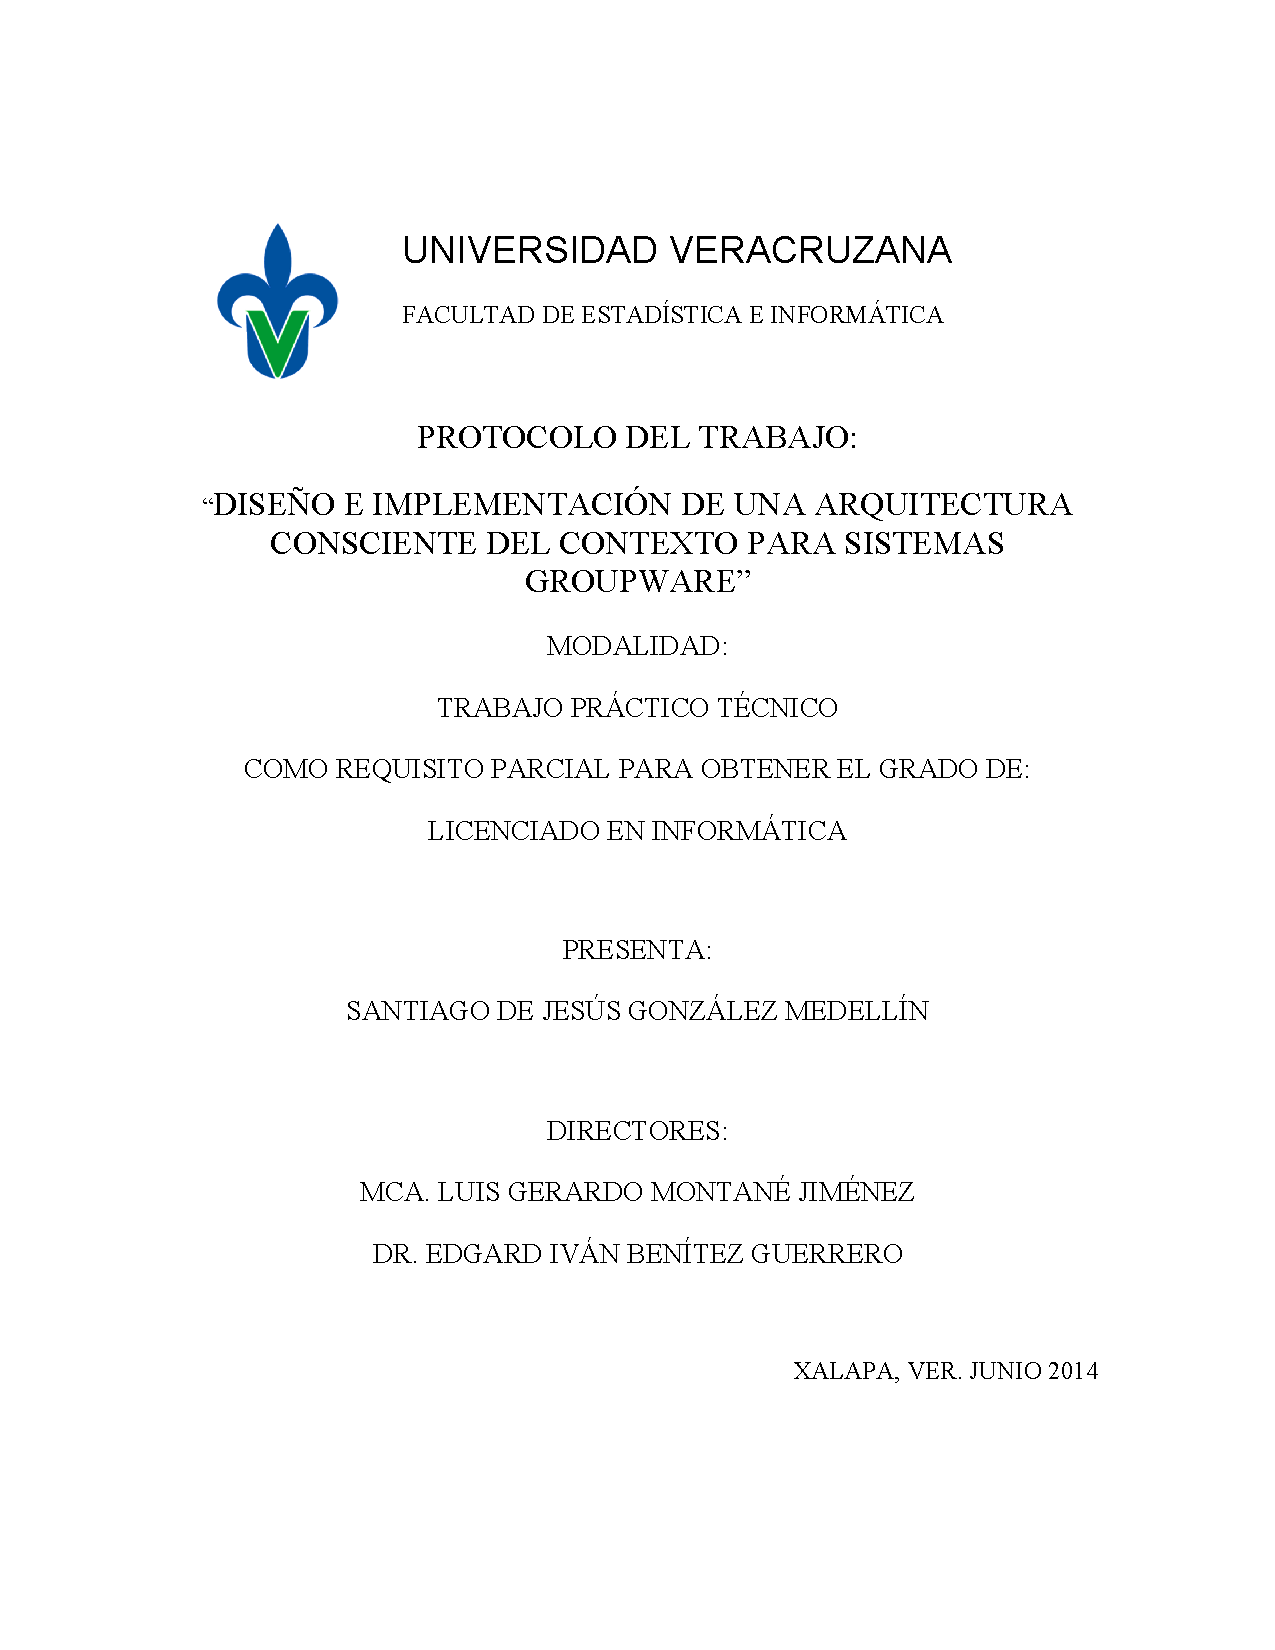
\includepdf{portada.pdf}
% %Resumen % %
\section*{Resumen}
El trabajo colaborativo es una actividad en la que un grupo de personas une sus esfuerzos para alcanzar un objetivo realizando tareas en las que otras personas pueden estar involucradas. El Trabajo Colaborativo Asistido por Computadora (CSCW) \footnote{CSCW por sus siglas en ingl\'es(\textit{Comupter Supported Collaborative Work})} es el \'area que estudia los sistemas computacionales que ayudan a estos grupos de trabajo a mejorar la coordinaci\'on, cooperaci\'on y comunicaci\'on que hay entre los integrantes del grupo de trabajo.

Entre los sistemas que estudia el CSCW se encuentran los Groupware, sistemas que fungen como medio para que los usuarios interact\'uen entre s\'i y puedan llevar a cabo tareas en conjunto. Para facilitar la interacci\'on de estos usuarios con el sistema y con otros usuarios, los groupware les proporcionan comunicaci\'on e informaci\'on para que tengan conocimiento de la situaci\'on actual con el fin de facilitar la toma de decisiones. As\'i surge la necesidad de dotar a los sistemas con el conocimiento necesario para poder proporcionar tales niveles de conscienca al usuario, a partir de esta necesidad se desarrollan sistemas conscientes del contexto. Los Sistemas Groupware Conscientes del Contexto (CAGS por sus siglas en ingl\'es)\footnote{ \textit{Context Aware Groupware Systems}} tienen ambas caracter\'isticas antes descritas: apoyan el trabajo colaborativo de un grupo de usuarios y soportan el uso de contexto y opera en consecuencia a esta informaci\'on, para eso se dise\~an arquitecturas conscientes del contexto que se integran a un groupware y puedan, entre ambos sistemas, funcionar como un CAGS. 

En el presente trabajo se hace una revisi\'on de las arquitecturas conscientes del contexto para analizar sus caracter\'isticas y poder dise\~nar una dirigida a sistemas groupware independiente del escenario en el que se desempe\~nen, la arquitectura parte de un trabajo antes propuesto\cite{montane2013context} en el que se divide el manejo de la informaci\'on contextual en 3 etapas: la recuperaci\'on de la informaci\'on, gesti\'on de los datos recuperados y el uso y distribuci\'on de resultados. Para la generaci\'on de CAGS es necesario un mecanismo de razonamiento contextual, el cual pueda generar resultados a partir de informaci\'on del contexto del sistema, para esto se propone un lenguaje de definici\'on de comportamiento del que se infieren dichos resultados, adem\'as se necesita implementar una ontolog\'ia o clasificaci\'on contextual que pueda ser reutilizada en cualquier caso de estudio. Una vez terminado el dise\~no se implementar\'a la arquitectura con un groupware y se har\'an pruebas.

Actualmente la mayor\'ia de las arquitecturas elaboradas est\'an orientadas a groupwares con ambientes espec\'ificos, es decir, usan el contexto de un escenario en particular, por ejemplo un sistema para  procesos empresariales, tomar\'ia en cuenta datos sobre el giro de la empresa y las actividades que se realizan internamente inherentes a las pol\'iticas de la organizaci\'on; estos datos no ser\'ian de utilidad para otro tipo de situaciones como en un groupware para desarrollo de software que se centra en los proyectos de desarrollo y que utiliza otro tipo de variables contextuales.
%\thispagestyle{electronic}
%%\newpage
%%M�rgenes
\marginsize{2.4cm}{2.4cm}{2.2cm}{2.5cm}
% Controla los m�rgenes {izquierda}{derecha}{arriba}{abajo}. 
\newpage
\begin{spacing}{1.5}
  \tableofcontents
\end{spacing}

\newpage
%\listoftables
%\listoffigures
%\newpage

%Para las pablabras cortadas
\clubpenalty=10000
\widowpenalty=10000
%\renewcommand{\baselinestretch}{1.20}
%\setlength{\parskip}{4mm}
%\pretolerance=2000
%\tolerance=3000
%\setlength{\parskip}{1ex plus 0.5ex minus 0.2ex}
\setlength{\parskip}{5mm}
\section{Introducci\'on}
\label{sec:intro}
Actualmente la mayor\'ia de las actividades, operaciones o procedimientos que se llevan a cabo en la industria, el entretenimiento y la vida diaria son desarrollados de manera conjunta, un grupo de personas unen sus esfuerzos para poder realizar diversas tareas. Tradicionalmente los sistemas de informaci\'on son un medio importante en muchas de estas tareas. El \'area que estudia estos sistemas es el Trabajo Colaborativo Asistido por Computadora o CSCW por sus siglas en ingl\'es (Computer Supported Collaborative Work). Entre los sistemas que estudia CSCW est\'an, en particular, los groupware, sistemas que apoyan a un grupo de trabajo proporcionando comunicaci\'on e informaci\'on a los usuarios sobre la actividad que se est\'an realizando, Ellis \cite{ellis1991groupware} define Groupware como sistemas computacionales que apoyan a grupos de personas ocupadas en una tarea en com\'un(u objetivo) y que proporcionan una interfaz para un ambiente compartido. Para hacer que la interacci\'on humano-computadora se lleve a cabo de manera m\'as natural y transparente, se dota al Groupware con la habilidad de percibir y trabajar con datos que describan la situaci\'on que rodea al grupo, esto se le conoce como consciencia contextual, una caracter\'istica que trae consigo el surgimiento de los Sistemas Groupware Conscientes del Contexto (CAGS).


Para que los Groupware Conscientes del Contexto(CAGS por sus siglas en ingl\'es) puedan trabajar con datos contextuales es necesario tener una descripci\'on del ambiente en el que va a trabajar, hace falta especificar los elementos que se deben de tomar en cuenta, por ejemplo, para un sistema de edici\'on simultanea de textos se debe trabajar informaci\'on como las modificaciones que se han hecho, la fecha de las modificaciones, los permisos de los usuarios tienen para acceder al documento, etc. mientras que para un sistema de gu\'ia de turistas se toman elementos como la ubicaci\'on del usuario, el lugar(por ejemplo un edificio, o en un espacio abierto), fechas de eventos pr\'oximos, etc. Como se puede observar en ambos casos, se usan descripciones diferentes del ambiente del sistema y esto implica tener que desarrollar 2 sistemas completamente diferentes, uno para cada caso en espec\'ifico. Esto se vuelve un problema al momento de desarrollar varios sistemas que requieren el procesamiento de informaci\'on contextual, ya que hay que estar cambiando la especificaci\'on del contexto cada vez y, en el peor caso, desarrollar desde cero un sistema para un ambiente completamente distinto de los creados anteriormente.

Para evitar este problema, se propone modelar e implementar una arquitectura orientada a servicios para sistemas groupware conscientes del contexto, cuyo dise\'no tome en cuenta los aspectos contextuales m\'as generales, est\'a arquitectura deber\'a poder utilizada en cualquier \'ambito reduciendo as\'i tiempo de desarrollo, ser\'a probada en un juego colaborativo (un videojuego de disparos en primera persona) y se documentar\'an los resultados para futuras investigaciones.


\section{Antecedentes}
Shmidt \cite{schmidt1992taking}, uno de los pioneros en el tema, define el trabajo colaborativo asistido por computadora (CSCW) como un \'area de investigaci\'on dirigida al dise\'no de sistemas de aplicaci\'on para una categor\'ia espec\'ifica de trabajo. Algunos de los sistemas que estudia esta \'area son los Groupware, sistemas de magnitud organizacional, que permiten la colaboraci\'on, comunicaci\'on y coordinaci\'on de un grupo para alcanzar una meta. Estos \'ultimos tres conceptos (colaboraci\'on, comunicaci\'on y coordinaci\'on) son de suma importancia para el trabajo colaborativo, para que estos sean llevados a cabo de manera eficiente es necesario que los miembros del grupo tengan conciencia de la situaci\'on en muchos niveles \cite{gutwin1996supporting}. 

En un groupware es dif\'icil que los usuarios tengan conciencia completa de todo el espacio de trabajo en el que participan, por ejemplo, disminuyendo las v\'ias de comunicaci\'on como  en la conciencia de un juego colaborativo \cite{montane2013context}, cuando los usuarios juegan en una misma habitaci\'on pueden comunicarse directamente con sus compa\'neros, ver sus expresiones, y percibir sus sentimientos; mientras que, al jugarlo en habitaciones distintas les es m\'as dif\'icil poder captar este tipo de se\'nales. Adem\'as de eso, para que el sistema pueda proveer medios de colaboraci\'on que permitan a los usuarios comunicarse eficientemente, ellos tienen que interactuar expl\'icitamente con los medios de comunicaci\'on que ofrece el sistema, provocando distracciones que afectan la concentraci\'on de los usuarios para lograr el objetivo principal. Para dar soluci\'on a este tipo de problemas en los groupware, se le proporciona al sistema informaci\'on del \'ambito en el que se ejecuta para poder hacerla consciente del contexto.
 
El c\'omputo consciente del contexto es un t\'ermino discutido por primera vez en el trabajo de Schilit y Theimer \cite{schillit1994disseminating} como software que se adapta de acuerdo al contexto, esto limita la definici\'on a aplicaciones que son informadas sobre el contexto y se adaptan a \'el, no dejando en claro qu\'e tipo de adaptaci\'on es la que realiza. En investigaciones m\'as recientes, Dey \cite{dey2001conceptual}, tomando como referencia investigaciones anteriores, define computaci\'on consciente del contexto como un sistema que usa el contexto para proporcionar informaci\'on relevante y/o servicios al usuario, donde la relevancia depende de la tarea del usuario. La definici\'on de Dey se puede ver reflejada en el ejemplo del sistema gu\'ia de turistas, donde la informaci\'on dada por el sistema es de inter\'es para los usuarios y la actividad que realizan, como por ejemplo, notificar de eventos pr\'oximos, o recomendar actividades o lugares a los turistas. En el caso de los videojuegos, el sistema ejecutar\'a instrucciones para ir aumentando la dificultad o el nivel del juego conforme el usuario va incrementando su habilidad, esto cumple la segunda propiedad de la definici\'on de Dey que es ejecutar un comando para adaptarse al contexto.

Se entiende por contexto la situaci\'on actual que tiene lugar en una actividad realizada por un sujeto o un grupo de entidades. Estas situaciones est\'an definidas por diferentes elementos que responden a las preguntas ?`qui\'en?, ?`d\'onde?, ?`cu\'ando? y ?`qu\'e?. Schilit y Theimer \cite{schillit1994disseminating} se refieren al contexto como la ubicaci\'on, identidades de personas y objetos cercanos, y los cambios en esos objetos. Mientras que la definici\'on de Dey \cite{dey2001conceptual} menciona que el contexto es cualquier informaci\'on relevante sobre las entidades en la interacci\'on entre el usuario y una computadora, incluy\'endolos a ambos, una entidad puede ser una persona, lugar u objeto considerado relevante para la interacci\'on entre un usuario y una aplicaci\'on.

\section{Definici\'on del problema}
En un ambiente colaborativo existe mucha interacci\'on entre los integrantes, necesitan estar comunic\'andose  constantemente para poder coordinar sus esfuerzos, y en un groupware es a\'un m\'as dif\'icil ya que el sistema se vuelve intermediario entre los usuarios,  para poder hacer estas interacciones m\'as fluidas el sistema necesita saber c\'omo ayudar a los usuarios y esto se logra d\'andole datos del contexto en general y logrando que razone y act\'ue  en beneficio del grupo.

Para que una aplicaci\'on pueda ser consciente del contexto, debe de ser capaz de adquirir informaci\'on contextual, gestionarla, y procesarla para obtener resultados que permitan ejecutar un comando o mostrar informaci\'on para el usuario. 

Se han propuesto muchos modelos y arquitecturas para el desarrollo de sistemas consientes del contexto, el problema de estos sistemas es que est\'an basados en escenarios particulares, es decir, satisfaciendo necesidades espec\'ificas del problema; por ejemplo, Meeting Reminder Agent\cite{anhalt2001toward}, toma el tiempo de distracci\'on de actividades, la ubicaci\'on, y el sonido en un campus para avisar al usuario de los lugares donde se est\'an llevando a cabo reuniones, y sugerir de acuerdo con los intereses del usuario, conferencias que se lleven a cabo. Otro caso es Portable Help Desk (PHD) \cite{anhalt2001toward} que es una aplicaci\'on que toma en cuenta la cercan\'ia de los miembros de un grupo y su disponibilidad para poder brindar apoyo a otros miembros y carecen de generalidad para poder ser aplicados en ambientes con un contexto diferente al que han sido desarrollados. Por \'ultimo CO2DE \cite{schmidt1992taking} que se concentra en la edici\'on colaborativa as\'incrona de diagramas y resoluci\'on de conflictos que mantiene el contexto individual de los integrantes del proyecto y evita traslapar ediciones manteniendo a cada contexto de los individuos en una rama diferente al proyecto original.

Se puede observar en los tres ejemplos anteriores que cada aplicaci\'on usa elementos diferentes del contexto seg\'un las necesidades que cubren, y si se quiere integrar el modelo de uno de ellos a otro \'ambito diferente, har\'ia falta integrar las caracter\'isticas que el anterior no ten\'ia, lo que supone una mayor carga en el modelado de soluciones. Por lo tanto, servicios fundamentales de contexto gen\'erico son requeridos para hacer de la conciencia del contexto una tecnolog\'ia factible que puede ser f\'acilmente incorporada a una variedad de software (Pascoe, J., Ryan, N., \& Morse, D., 1999).
 
Montan\'e \cite{montane2013context} propone una arquitectura para apoyar el trabajo colaborativo en los groupware en cuyos m\'odulos se pueden encontrar los elementos anteriores. La primera capa es de adquisici\'on de datos contextuales en la que cada m\'odulo trabaja con tipos diferentes de datos contextuales; en la capa de gesti\'on de contexto se almacena la informaci\'on obtenida en una base de datos para f\'acil acceso, aqu\'i se guardar\'an, actualizar\'an y recuperar\'an los datos hist\'oricos de la aplicaci\'on; en la \'ultima capa, que es la de uso de contexto, se encuentran 2 m\'odulos, uno que procesa y razona la informaci\'on contextual, y otro que entrega los resultados al sistema groupware.

Actualmente se encuentra desarrollada la capa de adquisici\'on de datos, pero para poder implementar la arquitectura en su totalidad, hacen falta desarrollar un modelo de las capas de gesti\'on de datos y de razonamiento contextual, de ah\'i el surgimiento del presente trabajo.

\section{Objetivos}
El fin principal de este trabajo es dise\~nar e implementar una arquitectura funcional orientada a servicios para sistemas Groupware consientes del contexto, particularmente en el caso de estudio de los videojuegos colaborativos, partiendo de un modelo propuesto anteriormente \cite{montane2013context}. Para poder llevar a cabo lo anterior se proponen los siguientes objetivos
\begin{itemize}
\item Implementar un modelo de consciencia contextual en el \'ambito de los videojuegos
\item Dise\~nar una arquitectura orientada a servicios para el uso, adquisici\'on y gesti\'on de informaci\'on contextual.
\item Desarrollar el m\'odulo de razonamiento contextual,  gesti\'on y realizar pruebas.
\item Integrar un m\'etodo de razonamiento contextual para ser aplicado en la capa de razonamiento.
\item Validar la arquitectura con el caso de estudio.
\end{itemize}
\section{Justificaci\'on}
La comunicaci\'on, coordinaci\'on y cooperaci\'on entre grupos colaborativos de trabajo es muy importante, con su eficiencia aumenta el rendimiento de los usuarios en el trabajo que realizan, fomentando la productividad. Con los groupware se mejora la calidad de operaci\'on de estos grupos, y a\'nadiendo la conciencia del contexto a este tipo de sistema, la interacci\'on que los usuarios tienen con los dispositivos o aplicaciones se hace de forma m\'as natural y fluida, permiti\'endoles concentrarse en la tarea que est\'an haciendo en lugar de detalles de comunicaci\'on y evitando la carga de procesamiento de informaci\'on que el sistema har\'a por ellos. Con la arquitectura que se va a dise\'nar, el desarrollo se vuelve menos complejo, evitando que los desarrolladores empiecen desde cero un proyecto que incluya groupware consciente del contexto.
\section{Alcances y Limitaciones}
Se pretende proponer una arquitectura gen\'erica orientada a servicios e implementarla en un sistema groupware, se extraer\'a informaci\'on contextual y se procesar\'a con un mecanismo tambi\'en propuesto, en la arquitectura se har\'a una distribuci\'on f\'isica y l\'ogica de cada uno de los m\'odulos de la arquitectura y se establecer\'an formas de comunicaci\'on entre ellos. Tambi\'en se implementar\'a una clasificaci\'on contextual que abarque los elementos necesarios para definir la situaci\'on de un ambiente. A pesar de que la arquitectura y el m\'etodo de razonamiento est\'a planteada para funcionar en cualquier caso de estudio, se probar\'a  por ahora en un videojuego colaborativo de disparos en primera persona, ambiente que nos proporciona equipos que compiten entre si para cumplir objetivos seg\'un el modo de juego.


\section{Marco Te\'orico}
\subsection{Trabajo colaborativo y Sistemas Groupware}

La mayor\'ia de las actividades que una persona realiza son en grupo \cite{ellis1991groupware}, para el apoyo a este tipo de actividades existen los sistemas groupware que son aquellos que apoyan a personas ocupadas en una tarea en com\'un, y que proveen una interfaz a un ambiente compartido, \cite{ellis1991groupware} cuyo objetivo es facilitar la comunicaci\'on, cooperaci\'on, y coordinaci\'on de los usuarios, seg\'un Cruz \cite{cruz2012towards} la comunicaci\'on se entiende como el proceso de interacci\'on entre personas que incluye el intercambio impl\'icito o expl\'icito de informaci\'on; Malone \& Crowston \cite{malone1994interdisciplinary} definieron coordinaci\'on como el manejo de interdependencias entre actividades realizadas por multiples actores basadas en objetos mutuos que son intercambiados entre actividades; la cooperaci\'on ocurre cuando un grupo trabaja para lograr una misma meta \cite{malone1994interdisciplinary} con alto grado de tareas interdependientes, compartiendo la informaci\'on disponible a trav\'es de alguna clase de espacio compartido. Existen diferentes tipos de sistemas groupware, \cite{ellis1991groupware} define 2 clasificaciones: por espacio-tiempo y por tipo de aplicaci\'on. Entre el rubro espacio-tiempo se encuentran aquellos que su funcionalidad permite interacciones cara a cara o interacciones distribuidas, as\'i mismo podemos encontrar aquellos que permiten una interacci\'on en tiempo real o una interacci\'on as\'incrona. Adem\'as de s\'incronos y as\'incronos agrega un tercer rubro que es la mixta que combina los dos anteriores, y engloba todos en la caracter\'istica de tipo de comunicaci\'on, y para la interacci\'on de los usuarios agrega la caracter\'istica de saber si el usuario est\'a conectado o desconectado en caso de las interacciones distribuidas, estas las incluye en la categor\'ia de disponibilidad del usuario\cite{antunes2014reviewing}.

Por otra parte cuando se toma en cuenta el tipo de aplicaci\'on para clasificar los sistemas groupware, podemos encontrar los siguientes: Sistemas de mensajes que soportan el intercambio as\'incrono de mensajes entre miembros de un grupo; editores multiusuario que permite a miembros de un grupo crear y editar un mismo documento al mismo tiempo, pueden ser s\'incronos o as\'incronos; sistemas para soporte de decisiones de grupo y cuartos electr\'onicos de reuniones, proveen infraestructura para la exploraci\'on de problemas no estructurados en un grupo; c\'omputo para conferencias: proporciona servicios como medios de comunicaci\'on en muchas formas, hay 3 tipos: de tiempo real, teleconferencia, y de escritorio; y por \'ultimo los agentes inteligentes que son programas computacionales \textit{inteligentes} encargados de tareas espec\'ificas.

Adem\'as de esta clasificaci\'on Ellis\cite{ellis1991groupware} propone elementos que tienen que ser tomados en cuenta para poder comparar y describir a los sistemas groupware, entre ellos se encuentran el contexto compartido que es el ambiente en el que va a correr el sistema; un grupo de ventanas que son las que se van a mostrar en diferentes pantallas del sistema y se van a compartir; un tele apuntador que es la capacidad de m\'as de un usuario de mover el apuntador al mismo tiempo; vista, es la porci\'on de contexto o ambiente que se va a mostrar en diferentes ventanas del sistema; sesi\'on que son los tipos de interacci\'on del usuario con el sistema y que ya se mencionaron antes (mismo tiempo, mismo lugar; diferente tiempo, diferente lugar, etc.) y los roles que son los tipos de usuarios que hay y los derechos y permisos que tienen con el sistema.

Shmidt \cite{schmidt1992taking} menciona varias propiedades que deben de tener los sistemas groupware:
\begin{itemize}
\item Es social; objeto, sujeto, medios, fines, motivos y necesidades, competencias e implementaciones, est\'an mediadas socialmente.
\item Integrantes mutuamente dependientes, necesitan cooperar para terminar el trabajo. Diferente a solo compartir el mismo recurso, sujeto A conf\'ia positivamente en la calidad y l\'ineas de tiempo del trabajo de sujeto B y vice versa
\item Distribuci\'on de tareas qu\'e va a hacer cada individuo, cu\'ando y d\'onde.
\item Distribuci\'on f\'isica en tiempo y espacio
\item Distribuci\'on l\'ogica, en t\'erminos de control, en el sentido de que los sistemas son semi aut\'onomos en su trabajo parcial.
\item Deben aumentar las capacidades mec\'anicas y de procesamiento de informaci\'on del individuo.
\item Deben combinar las actividades especializadas de m\'ultiples trabajadores dedicados a las diferentes herramientas especializadas.
\item Deben facilitar las aplicaciones de m\'ultiples problemas resolviendo estrategias y heur\'isticas de un problema dado.
\item Deben facilitar la aplicaci\'on de m\'ultiples perspectivas y concepciones de un problema dado para adaptarse a naturaleza m\'ultiple del ambiente de trabajo.
\item Deben apoyar la auto organizaci\'on, de conjuntos cooperativos al contrario de interrumpir trabajo cooperativo computarizando procedimientos formales.
\end{itemize}

Para Shmidt \cite{schmidt1992taking} el trabajo colaborativo es siempre social, en el sentido en el que el objeto y el sujeto, los fines y los medios, los motivos y necesidades est\'an mediados socialmente, cada elemento del grupo depende, en parte, del trabajo de alg\'un otro miembro y viceversa, y cuando esto sucede, es importante que ambos elementos del grupo tengan el conocimiento de los avances del otro para poder hacer una estimaci\'on de sus propias acciones, esto es, que cada miembro tenga conciencia de lo que pasa a su alrededor para que pueda tomar demisiones adecuadas en cuanto a la actividad que tiene asignada en el grupo.

\subsection{Consciencia}

Gutwin \cite{gutwin1996supporting} menciona que es importante que los individuos sepan lo que est\'an haciendo los dem\'as ya que pueden usar ese conocimiento para anticipar las acciones de los otros, y ayudarlos con sus tareas, Dourish y Bellotti \cite{dourish1992awareness} fueron los primeros en introducir el t\'ermino awareness diciendo que es el entendimiento de las actividades de otros, que proporciona un contexto para tu propia actividad, a\'un m\'as, dicen que este contexto es usado para asegurar que las contribuciones individuales sean relevantes a las actividades del grupo como un todo, y para evaluar las acciones individuales con respecto a los objetivos del grupo y progresos. 

En un estudio realizado por \cite{Belkadi2013110} se mencionan las caracter\'isticas que debe de tener la consciencia o el conocimiento, entre ellas se encuentran el tener muchas facetas, es decir, existen diferentes tipos de conocimiento como se explicar\'a m\'as adelante; el conocimiento est\'a fuertemente enlazado a situaciones colaborativas ya que los colaboradores necesitan informaci\'on para llevar a cabo algunas tareas o para tomar decisiones; el conocimiento en una situaci\'on colaborativa puede incrementar los niveles de confianza entre actores lo que los alienta a compartir informaci\'on. Adem\'as de estas caracter\'isticas proponen 3 tipos de conocimiento, o consciencia: Consciencia social, Consciencia de las tareas y Consciencia del espacio de trabajo; estas tres categor\'ias se pueden identificar con las preguntas de la siguiente tabla:

\begin{center}
\begin{longtable}{|p{2cm}|p{11cm}|}
\caption{Preguntas para entender los tipos de consciencia.}\\
\hline
\textbf{Tipo de consciencia} & \textbf{Preguntas}\\
\hline
\endfirsthead
\multicolumn{2}{c}%
{\tablename\ \thetable\ -- \textit{Contin\'ua de p\'agina anterior}} \\
\hline
\textbf{Tipo de consciencia} & \textbf{Preguntas} \\
\hline
\endhead
\hline \multicolumn{2}{r}{\textit{Contin\'ua en siguiente p\'agina}} \\
\endfoot
\hline
\endlastfoot

	Consciencia Social & ?`Qu\'e debo de esperar de otros miembros del grupo? ?`C\'omo voy a interactuar con el grupo? ?`Qu\'e rol voy a tomar en este grupo? ?`Qu\'e roles van a tomar los dem\'as miembros del grupo? \tabularnewline \hline
	Consciencia de las Tareas & ?`Qu\'e s\'e de este tema y la estructura de la tarea? ?`Qu\'e saben los dem\'as? ?`Qu\'e se necesita para completar la tarea? ?`C\'omo ser\'an evaluados los resultados? ?`Qu\'e herramientas u objetos se necesitan para completar esta tarea? ?`Cu\'anto tiempo se necesita y cu\'anto tiempo hay disponible? \tabularnewline \hline	
	Consciencia del espacio de trabajo & ?`Qu\'e hacen los dem\'as miembros del grupo para completar la tarea? ?`D\'onde est\'an? ?`Est\'an activos en el espacio de trabajo? ?`Qu\'e har\'an? ?`Qu\'e hacen actualmente? ?`Qu\'e han hecho? ?`Qu\'e har\'an despu\'es? ?`C\'omo los puedo ayudar? \tabularnewline
	\hline
\end{longtable}
\end{center}

Por otro lado  \cite{antunes2014reviewing} identifica seis tipos diferentes de consciencia; la consciencia colaborativa, la consciencia contextual, consciencia social, consciencia del espacio de trabajo, consciencia situacional, y consciencia del lugar.

\subsubsection{Consciencia colaborativa}

Ha sido generalmente aceptado como la percepci\'on de la disponibilidad del grupo que tiene cada uno de los integrantes. Disponibilidad del grupo quiere decir el conocimiento de si las personas est\'an en el mismo lugar f\'isico, o si est\'an conectados o desconectados y los medios de comunicaci\'on que tienen disponibles para colaborar entre s\'i.

\subsubsection{Conciencia contextual}

La conciencia contextual es fundamental para permitir que un grupo colaborativo tenga conocimiento de lo que est\'a pasando en el espacio virtual del sistema.

\subsubsection{Conciencia social}

La conciencia social \cite{antunes2014reviewing} apunta la importancia de entender las pr\'acticas sociales, como los roles de otros y sus actividades, o c\'omo est\'an otros miembros del grupo contribuyendo a una tarea.

\subsubsection{Conciencia de espacio de trabajo}

La conciencia del espacio de trabajo se divide en 2 aspectos: uno se enfoca en el lugar y el otro se enfoca en el espacio, otra cosa importante a considerar es la interacci\'on del grupo con los lugares de trabajo, finalmente la noci\'on del espacio de trabajo trae consigo el nivel de interdependencia de una tarea realizada por el grupo, considerando soporte de actividades paralelas, actividades coordinadas y actividades mutuamente ajustadas.

\subsubsection{Conciencia situacional}

Est\'a caracterizado por tres niveles cognitivos: en el primero una percepci\'on global del ambiente construido por eventos, acciones, recursos y otros elementos, en el segundo nivel se le da un sentido a lo que est\'a pasando actualmente y en el tercero se construyen escenarios a futuro.

\subsubsection{Conciencia del lugar}

Puede referirse al conocimiento de los elementos de una ubicaci\'on geogr\'afica como pueden ser coordenadas, orientaci\'on, distancia, etc. O tambi\'en el conocimiento de los elementos de un espacio f\'isico, incluyendo clima, topolog\'ia f\'isica del lugar, y atributos f\'isicos.

\newpage
\subsection*{}


Por la naturaleza de los sistemas groupware las \'areas de m\'as inter\'es son la conciencia social y la conciencia del espacio de trabajo. En otra clasificaci\'on (Gutwin, C., Greenberg, S., \& Roseman, M., 1996) podemos encontrar 2 tipos de conciencia al contexto: primero conciencia general de las personas en una comunidad de trabajo, y segundo conciencia de las interacciones de otros en un espacio compartido.

Gutwin (Gutwin, Carl, Greenberg, Saul 1996) propone un marco de trabajo que considera elementos que incluyen mecanismos para recolectar informaci\'on \'util para la conciencia de la situaci\'on por parte de las personas, y que integran el conocimiento consciente del espacio de trabajo de un grupo.

\begin{center}
\begin{longtable}{|l|p{8cm}|}
\caption{Elementos de conciencia de la situaci\'on propuestos por Gutwin\cite{gutwin1996supporting}}\\
\hline
\textbf{Elementos} & \textbf{Cuestiones que responden}\\
\hline
\endfirsthead
\multicolumn{2}{c}%
{\tablename\ \thetable\ -- \textit{Contin\'ua de p\'agina anterior}} \\
\hline
\textbf{Elementos} & \textbf{Cuestiones que responden} \\
\hline
\endhead
\hline \multicolumn{2}{r}{\textit{Contin\'ua en siguiente p\'agina}} \\
\endfoot
\hline
\endlastfoot

Presencia & ?`Qui\'enes est\'an participando en la actividad?\\
Ubicaci\'on & ?`D\'onde est\'an trabajando?\\
Nivel de actividad & ?`Qu\'e tan activos son en el espacio de trabajo?\\
Acciones & ?`Cu\'ales son sus actividades y tareas actuales?\\
Intenciones & ?`Qu\'e har\'an despu\'es?, ?`D\'onde van a estar?\\
Cambios & ?`Qu\'e cambios est\'an realizando y en d\'onde?\\
Objetos & ?`Qu\'e objetos est\'an usando?\\
Extensiones & ?`Qu\'e pueden ver?, ?`Cu\'ales son sus alcances?\\
Habilidades & ?`Qu\'e pueden hacer?\\
Esfera de influencia & ?`D\'onde pueden hacer cambios?\\
Expectativas & ?`Qu\' se necesita que haga ahora?\\
\hline
\end{longtable}
\label{elem:context}
\end{center}

Todos los elementos de la tabla \ref*{elem:context} se pueden clasificar en dos grupos: aquellos que se encargan de saber que est\'a pasando con otras personas, y aquellos que se encargan de saber d\'onde est\'a pasando. Esta clasificaci\'on detalla el perfil individual de cada integrante y sigue las actividades de cada uno. En otro caso, en el trabajo de Montan\'e \cite{montane2013context} se propone un modelo de contexto social, donde hay categor\'ias similares, pero tomando en cuenta las relaciones entre los sujetos adem\'as de las actividades y estado actual de cada uno de ellos, los elementos que lista en su trabajo est\'an divididos en tres categor\'ias. La interactiva describe a los usuarios de forma individual y sus interacciones con las cosas que los rodean como objetos, tareas, eventos, usuarios o ubicaciones; la cohesiva integra elementos que tienen que ver con la actividad grupal y se pueden encontrar los grupos, roles, metas, alianzas, actividades y reglas. Y las afectivas que describe c\'omo se sienten los miembros del grupo al realizar las actividades entre ellas est\'an los sentimientos y los gestos.

\subsection{Consciencia del contexto}
Todos los elementos antes mencionados hacen referencia a la conciencia de parte del usuario del contexto que lo rodea, pero ?´es posible hacer que la conciencia del ambiente pueda ser aprendida por el propio sistema groupware? Existen sistemas groupware que son capaces de reconocer aspectos contextuales que rodean a un grupo de usuarios, estos sistemas son llamados conscientes del contexto, la informaci\'on contextual m\'as com\'un en los sistemas groupware es la ubicaci\'on f\'isica del usuario. Al hablar de sistemas groupware conscientes del contexto surgen algunos asuntos importantes que estos han de tomar en cuenta. Para empezar hace falta una categorizaci\'on formal del contexto en el que van a trabajar, el problema de esto es que los sistemas son desarrollados para que funcionen en \'ambitos espec\'ificos al problema o situaci\'on a la que se le quiere dar soluci\'on.

El conocimiento contextual describe una situaci\'on, la forma en la que se usan los elementos en un grupo de trabajo, incluyendo los eventos que son manejados por el grupo \cite{brezillon2004context}. Varios autores tienen un concepto de contexto algunos de ellos traslapan en definici\'on con otros, y diferentes elementos son tomados en cuenta para la descripci\'on de contexto. Dey \cite{dey2001conceptual} toma varias definiciones de contexto que otros autores hab\'ian hecho antes y hace su definici\'on que est\'a enfocada en el contexto en la computaci\'on, dice que contexto como cualquier tipo de informaci\'on que se puede usar para caracterizar la situaci\'on de entidades (se entiende por entidad una persona, lugar u objeto) que es considerada relevante para la interacci\'on entre un usuario y una aplicaci\'on incluyendo al usuario y la aplicaci\'on mismos.

Malik \cite{malik2007future} hace referencia a varios problemas que hay en la actualidad inherentes a consciencia contextual, entre ellos est\'an la definici\'on del contexto, ya que contexto es un concepto que abarca todos los posibles par\'ametros que identifican una situaci\'on, las aplicaciones y marcos de trabajo est\'an limitados a definir los par\'ametros del contexto de su propio \'ambito. Otro problema importante es que las arquitecturas no est\'an demasiado desarrolladas aun, est\'an desarrolladas para tareas espec\'ificas, hace falta est\'andares para definir una arquitectura y herramientas, por \'ultimo otro problema que es de inter\'es para este trabajo es la interpretaci\'on del contexto y las adaptaciones del comportamiento del servicio. 

Br\'ezillon \cite{brezillon2004context} estudia 3 casos de sistemas groupware conscientes al contexto y describe la forma en que apoya a la conciencia del contexto con los usuarios. SisPro es un sistema que tiene por objetivo facilitar las actividades colaborativas y procesos de aprendizaje y el desarrollo de competencias de trabajo colaborativo. SISCO tiene como tarea la preparaci\'on de reuniones,  da a conocer a los usuarios los temas de los que se est\'a hablando basados en su agenda individual. CO2DE es un software que permite unir los contextos individuales en un solo diagrama proporcionando una infraestructura de edici\'on colaborativa. Otro caso de sistema groupware muy diferente a los anteriores es Assault Cube \cite{montane2013context}, un juego FPS (Fisrt Shoter Person) de c\'odigo abierto que soporta las actividades colaborativas, en este varios jugadores se conectan a un servidor para llevar a cabo actividades espec\'ificas de la modalidad del juego que hayan escojido, el juego ofrece mecanismos de conciencia a los jugadores tales como un mapa de la ubicaci\'on del enemigo, un medidor de vitalidad, una pantalla de mensajes para comunicar al equipo, etc.

En figura 1 Se realiza una comparaci\'on tomando en cuenta los sistemas anteriores, para poder realizar las comparaciones se listan algunos aspectos propuestos por Gutwin \cite{gutwin1996supporting}, Montan\'e \cite{montane2013context}, Dey \cite{dey2001conceptual} y se clasifican en rubros m\'as grandes propuestos por Dey en otro de sus trabajos que son ambiente de usuario y ambiente f\'isico, el ambiente computacional, aunque es introducido por Dey, no es tomado en cuenta en ninguno de los sistemas ni en otras clasificaciones, as\'i que es omitido.

\begin{figure}[h!]
  \centering
    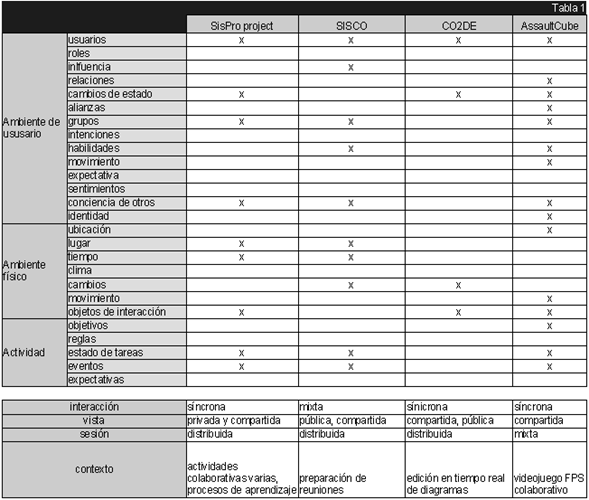
\includegraphics[scale=0.9]{groupware}
  \caption{Comparaci\'on de sistemas groupware}
  \label{cmp:gw}
\end{figure}

Como se puede observar en la figura \ref{cmp:gw} no todos los sistemas abarcan los mismos aspectos contextuales, cada uno tiene una arquitectura singular creada para satisfacer las necesidades del entorno para el que fueron creadas. 

En este trabajo se hace una propuesta de una arquitectura que pueda integrarse en cualquier tipo de sistema. Esta arquitectura tendr\'a soporte para el ambiente de aplicaciones ya que al ser el sistema groupware una entidad en el trabajo colaborativo, tiene que tener conciencia de s\'i misma y de otros sistemas que la rodean, incluyendo servicios, dispositivos, sensores, etc.


\section{M\'etodo}
Para este trabajo se estiman las siguientes actividades:

Fase 1:

Se revisar\'a el estado del arte de las arquitecturas para sistemas conscientes del contexto

Fase 2:

Se har\'a una investigaci\'on de las propiedades y elementos de los sistemas colaborativos e indagar como se puede establecer una comunicaci\'on con ellos para poder extraer y enviar los datos contextuales y resultados del procesamiento

Fase 3: 

Clasificaci\'on de contexto de manera general, para empezar a planear la forma de procesarlo, de esto saldr\'a un modelo conceptual de contexto en el que se basar\'a el desarrollo de la arquitectura antes propuesta.

Fase 4:

Distribuci\'on l\'ogica de m\'odulos de operaci\'on que participaran en el procesamiento de la informaci\'on contextual, producto de esto ser\'a un modelo de flujo de datos de los m\'odulos propuestos. Modelo de comunicaci\'on basado en servicios y se distribuci\'on de m\'odulos en distintos servidores para empezar a estructurar la arquitectura.

Fase 5:

Codificaci\'on de m\'odulos para empezar a implementar la arquitectura ya propuesta, se probaran los m\'odulos por separado y en conjunto para determinar la efectividad del producto. Aplicaci\'on de la arquitectura a un sistema groupware para realizar un caso de estudio, el sistema es un juego FPS (first person shoter) de c\'odigo abierto, en particular AssaultCube. Documentaci\'on de los resultados y conclusi\'on.

\section{Modelos Contextuales}

Contexto es tradicionalmente la localizaci\'on, identidad, y estado de las personas, grupos y objetos virtuales y f\'isicos, seg\'un Pereira  \cite{pereira2013CSCWD} el contexto puede ser visto como un conjunto de condiciones e influencias en una situaci\'on relevante y que la hacen \'unica y comprensible, esta situaci\'on puede referirse a una persona, grupo de personas, objeto f\'isico, entidad computacional, etc. El concepto de modelos mentales tiene una relaci\'on muy cercana a la consciencia contextual y situacional \cite{aehnelt2012discussion}, al momento de modelar contexto, es necesario distinguir entre los diferentes tipos de informaci\'on contextual\cite{hoyos2013domain}, el contexto de las actividades colaborativas pueden ir desde un editor de documentos distribuido, hasta un videojuego colaborativo; por lo que los elementos particulares de dichas actividades cambia muy radicalmente de uno a otro, y con esto surge la necesidad de usar una taxonom\'ia con un alto nivel de abstracci\'on que soporte la diversidad de contexto con los que se trabaja.

Belkadi et al \cite{Belkadi2013110} proponen un modelo situacional para mejorar la conciencia centrada en los conceptos de situaci\'on, interacci\'on y rol, en el que hacen un recuento de los conceptos clave a tomar en cuenta para un modelo, entre ellos se encuentran: 
\begin{itemize}
\item Elemento contextual
\item Tarea y actividad: describen lo que se espera y lo que se tiene que hacer.
\item Recursos: describe un elemento del contexto, en d\'onde es usado y c\'omo contribuye a la tarea.
\item Interacci\'on: interacciones entre un sujeto y un objeto mediante el uso de herramientas, e interacciones sociales mediante la definici\'on de reglas.
\item Role: definen las responsabilidades de los sujetos.
\end{itemize}

En su modelo para descripci\'on de situaciones definen entidades b\'asicas como recursos humanos y objetos, entidades de interacci\'on que relaciona a las entidades b\'asicas, las cuales se clasifican en cuatro tipos: operacional, que se refiere a las diferentes metas para ser cumplidas(tarea, actividad, proyecto); comunidad, que se refiere a la afiliaci\'on de unas entidades con otras; colaborativa que denota el intercambio de informaci\'on durante una actividad colectiva, y restricciones que indican requerimientos, reglas y l\'imites para la realizaci\'on de una tarea. En cuanto a los roles se definen cinco tipos: actor(\textquestiondown Qui\'en hace qu\'e ?), customer(\textquestiondown Para qui\'en ?), manager(\textquestiondown C\'omo ?), support(\textquestiondown Con qu\'e ?), object(\textquestiondown Sobre qu\'e ?).

As\'i mismo Pereira et. al. \cite{pereira2013CSCWD} maneja un modelo llamado SeCoM(\textit{Semantic Context Model}) dividida en tres capas: ontolog\'ia de alto nivel que representan el contexto o procesos de software, la  ontolog\'ia de integraci\'on es parte de una t\'ecnica para conectar los datos recojidos por los sensores con la arquitectura y la ontolog\'ia de sensores que implementan ontolog\'ias para los datos que son recolectados. El modelo SeCoM consiste de un conjunto modular de ontolog\'ias basadas en dimensiones sem\'anticas de identidad(Actor), ubicaci\'on(Espacio), temporal(tiempo), de actividad(Actividad) y m\'etodos de captura y acceso(Dispositivo).

En otro estudio Alves \cite{alves2013radiator} menciona una definici\'on para los elementos de su modelo definida formalmente como sigue: Un atributo $A_{i}$ es una tupla $( N, V )$, donde \textit{N} es un nombre representando el atributo(por ejemplo, velocidad) y $V$ es el valor del atributo(e.g., 100); $P$ es un conjunto finito de personas ${P_{1},P_{2}...P_{n}}$; $t$ es el rango de tiempo entre dos marcas de tiempo; y $\textit{A}$ un conjunto finito de atributos ${A_{1},A_{2}...A_{n}}$. Con estos elementos representa situaciones definiendo un contexto \textit{C} como una 3-tupla $( P, t, A )$ que representa los atributos que caracteriza la situaci\'on de un grupo de personas $P$ durante un intervalo de tiempo $t$. Por ejemplo suponiendo que Alice est\'a en Nueva York entre Julio 1 y Julio 3. Podemos definir su contexto $C$ como:

$C=( ( Alice ), 01/07..03/07, ( Ubicacion, Nueva York ))$

Este modelo esta orientado a la propagaci\'on despu\'es de que la informaci\'on ha sido agregada tomando en cuenta los atributos en com\'un de las personas que comparten un mismo contexto.

En el trabajo de Ardissono \cite{ardissono2012context} mencionan activity frames para simplificar el contexto de actividades cooperativas, un frame era definido por una 5-tupla $( fn, U, O, Oi, T )$, donde $fn$ era el nombre del frame, $U$ el conjunto de usuarios involucrados en la actividad, $O$ los objetos asociados al frame, $Oi$ es el conjunto de objetos del frame por medio de inferencias, y $T$ las tareas asociadas a la actividad. Y a su vez las tareas est\'an formadas por $( tn, U, O, Oi, g, P, T, s, d )$, donde $tn$ es el nombre de la tarea, $U$, $O$ y $Oi$ como dicho antes son los Usuarios, Objetos, y objetos inferidos asociados a la tarea, $g$ es el objetivo, $P$ es el grupo de tareas que deben de estar cerradas antes de iniciar $tn$, $T$ es el conjunto de tareas hijas, $s$ es el estado(habilitada, deshabilitada, cerrada) y $d$ es la fecha l\'imite para terminar la tarea, nula por defecto.

Anallely Olivares \cite{olivares2011} menciona que es importante tomar en cuenta el contexto de una actvidad colaborativa en lugar de hacerlo para cada uno de los usuarios, es por eso que en su modelo enfatiza el uso de variables t\'ipicas de un grupo de trabajo, por ejemplo estado de los proyectos, pol\'iticas de la organizaci\'on, ubicaci\'on f\'isica de los colaboradores, recursos disponibles, etc.

Bo Hu \cite{bohu2013} divide su modelo en dos partes una meta ontolog\'ia y una ontolog\'ia de dominio,  los elementos del meta modelo se encuentran organizados en cinco categor\'ias: c\'omputo, que define elementos como dispositivos, servicios, redes, y sistemas; persona, con elementos como usuarios, dise\~nadores y desarrolladores; ubicaci\'on, que se divide en la ubicaci\'on f\'isica y distancia; actividad, con dos tipos de actividades, planeadas y no planeadas; y misi\'on, donde se identifican misiones, metas y requerimientos. La ontolog\'ia espec\'ifica de dominio define los conceptos y relaciones dentro del dominio dado, y es restringido por el meta modelo.

En el a\~no 2013 se propone MARS que es un modelo contextual de regulaci\'on que ayuda a modelar la actividad soportada por herramientas groupware. En este modelo las interacciones toman lugar en un espacio llamado arena, cada interacci\'on es representada por un escenario que describe la forma en que se lleva a cabo dicha interacci\'on, qui\'enes participan y los objetos involucrados, adem\'as se definen condiciones y precondiciones para que este escenario se lleve a cabo; en esta arena est\'an presentes actores que realizan acciones, durante esta actividad se manejan o producen objetos; actores y objetos pertenecen a diferentes familias y desempe\'nan diferentes papeles o roles. Dado que los miembros de un grupo colaborativo pueden serlo a su vez de otro, se definen vistas que determinan los actores, objetos e interacciones que una arena puede compartir con otra.

En otro caso Montan\'e et. al. proponen un modelo de contexto social\cite{montane2013context}, donde hay categor\'ias similares, tomando en cuenta las relaciones entre los sujetos adem\'as de las actividades y estado actual de cada uno de ellos; los elementos que lista en su trabajo est\'an divididos en tres categor\'ias. La interactiva describe a los usuarios de forma individual y sus interacciones con las cosas que los rodean como objetos, tareas, eventos, usuarios o ubicaciones; la cohesiva integra elementos que tienen que ver con la actividad grupal y se pueden encontrar los grupos, roles, metas, alianzas, actividades y reglas. Y las afectivas que describen c\'omo se sienten los miembros del grupo al realizar las actividades entre ellas est\'an los sentimientos y los gestos.	

Skillen \cite{Skillen201497} habla de un mecanismo de personalizaci\'on basado en reglas donde identifica conceptos clave para modelar a los usuarios en un ambiente pervasivo de los que lista los siguientes: Usuario, Perfil de usuario, ubicaci\'on, preferencias del usuario, Objeto de asistencia en una interacci\'on, actividad que realiza el usuario, contenido multimedia que ser\'a enviado al usuario(audio, video, imagen o texto), Condici\'on de salud que pueden afectar el tipo de medio que se le env\'ia al usuario, escala de calidad de la informaci\'on entregada, y formato de interfaz de usuario donde se desplegar\'a la informaci\'on enviada.

En una revisi\'on de la literatura sobre modelos contextuales se revisaron ontolog\'ias contextuales, entre las que se pod\'ian encontrar los siguientes elementos:

\begin{center}
\begin{longtable}{|p{3cm}|p{10cm}|}
\caption{Unidades contextuales encontradas en los frameworks revisados.}\\
\hline
\textbf{Elementos} & \textbf{Descripci\'on}\\
\hline
\endfirsthead
\multicolumn{2}{c}%
{\tablename\ \thetable\ -- \textit{Contin\'ua de p\'agina anterior}} \\
\hline
\textbf{Elementos} & \textbf{Descripci\'on} \\
\hline
\endhead
\hline \multicolumn{2}{r}{\textit{Contin\'ua en siguiente p\'agina}} \\
\endfoot
\hline
\endlastfoot

	Objetos o artefactos & Entidades sobre las que los usuarios pueden realizar alguna acci\'on. \\
	\hline
	Tareas & Acciones asociadas con usuarios, objetos, objetivos y subtareas que se deben de llevar a cabo para alcanzar un objetivo. \\
	\hline
	Eventos & Eventos ocurridos en interacciones\cite{montane2013context}\\
	\hline
	Usuarios & Entidades que pertenecen a una comunidad y que realizan tareas\cite{montane2013context}. \\
	\hline
	Ubicaciones & Posici\'on virtual o f\'isica en un grupo \cite{montane2013context}. \\
	\hline
	Grupos & Colecci\'on de usuarios que realizan una actividad\cite{montane2013context}. \\
	\hline
	Objetivos & Los objetivos de la comunidad\cite{montane2013context}. \\
	\hline
	Alianzas & Subconjunto de usuarios en un grupo \cite{montane2013context}. \\
	\hline
	Actividades & Actividades realizadas por un grupo\cite{montane2013context}. \\
	\hline
	Reglas & Comportamientos definidos por el grupo \cite{montane2013context}. \\
	\hline
	Foco de visi\'on & D\'onde est\'an mirando los usuarios\cite{gallardo2012framework}. \\
	\hline
	Vistas de sistema, espacios de trabajo & Qu\'e pueden ver los usuarios \cite{gallardo2012framework}. \\
	\hline
	Alcance & Alcance de los usuarios\cite{gallardo2012framework}. \\
	\hline
	Presencia & Presencia de usuarios en el espacio de trabajo\cite{gallardo2012framework}. \\
	\hline
	Intenci\'on & De qu\'e objetivo es parte una tarea\cite{gallardo2012framework}. \\
	\hline
	Habilidades & Capacidad para llevar a cabo un conjunto de actividades con cierto nivel de destreza \cite{decouchant2013adapting}. \\
	\hline
	Contexto f\'isico & Incluye todas las magnitudes f\'isicas (e.g. tiempo, espacio, temperatura, nivel de luz, nivel de ruido)\cite{hoyos2013domain}. \\
	\hline
	Contexto computacional & Informaci\'on relacionada con el software y hardware de sistemas, e.g. trafico de red, condiciones, estatus de hardware, informaci\'on pedida por el usuario, requerimientos de memoria\cite{hoyos2013domain}. \\
	\hline
	Ambiente & Descripci\'on de la distribuci\'on f\'isica de los objetos y usuarios en un espacio de trabajo\cite{hoyos2013domain}. \\
	\hline
\end{longtable}
\end{center}

Todos estos elementos se extrajeron de diferentes modelos entre los que se hizo la siguiente tabla comparativa:

\begin{figure}[h!]
  \centering
    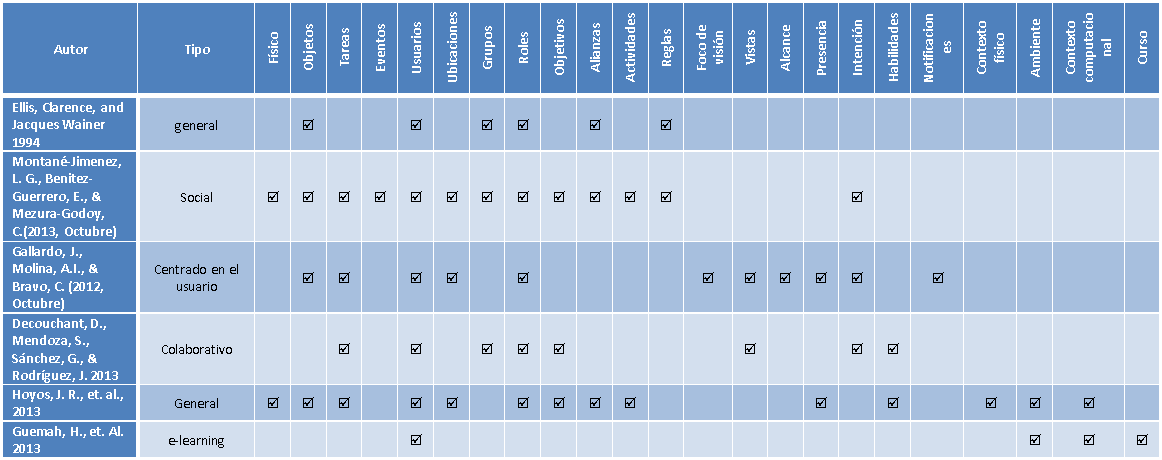
\includegraphics[scale=0.5]{cmpcntx}
  \caption{Comparaci\'on de modelos de contexto\cite{ellis1994conceptual}\cite{montane2013context}\cite{gallardo2012framework}}
\end{figure}

% % % % % % % % % % % % % % % % % % % % % % % % % % % % % % % % % % % % % % % % % % % % % % % % % % % % % % % % % % % % %

\section{Arquitecturas y Marcos de Trabajo Conscientes del Contexto}

Gutheim \cite{gutheim2011} menciona que hay dos tipos de arquitecturas, las que siguen un modelo distribuido haciendo uso de servicios(\textit{broker}) usado tradicionalmente para decoplar proveedores y consumidores de datos contextuales, este modelo es usualmente utilizado para  modelar contexto y para mecanismos de inferencia; el otro tipo de arquitecturas son aquellas que siguen un modelo punto a punto en el que generalmente los proveedores y consumidores de informaci\'on contextual se conocen mutuamente y se env\'ian informaci\'on directamente \cite{yoosoo2010}.

Para que una arquitectura sea consciente del contexto debe de cumplir con los siguientes requerimientos\cite{dey1999architecture}:

\begin{itemize}
\item Permitir a las aplicaciones acceder a informaci\'on contextual desde m\'aquinas distribuidas en el de la misma forma en que acceden a la entrada del usuario en una m\'aquina local.
\item Soportar la ejecuci\'on de diferentes plataformas y el uso de diferentes lenguajes de programaci\'on.
\item Soportar la interpretaci\'on de informaci\'on contextual.
\item Soportar la agregaci\'on de informaci\'on contextual
\item Soportar independencia y persistencia de widgets contextuales
\item Soportar el almacenamiento del historial de contexto
\end{itemize}

Tambi\'en para el soporte de consciencia contextual, Elg Ghayam \cite{el2011distributed} menciona 2 requerimientos que se deben de cumplir: la formalizaci\'on de contexto, para delimitar los datos contextuales y facilitar la distinci\'on de par\'ametros de contexto, una categorizaci\'on de datos contextuales es requerida, m\'as aun, para reducir la complejidad de su manutenci\'on, una representaci\'on formal tambi\'en es necesaria. El otro punto son reglas de adaptaci\'on: la adaptaci\'on de contexto debe de ser vista como un conjunto de reglas que controlan y anticipan el cambio de contexto que puede ocurrir en el ambiente, por lo tanto, en la construcci\'on de reglas de adaptaci\'on, el n\'umero de par\'ametros contextuales es grande y as\'i, no es evidente que no se pueden enumerar todas las posibles situaciones que van a ocurrir. Por lo anterior, un m\'etodo para construir reglas de adaptaci\'on es requerido, que pueda manejar la diversidad de posibles situaciones que se construyen en base de esos par\'ametros contextuales.

Para poder mejorar la colaboraci\'on de los usuarios, la arquitectura debe de permitir que el groupware pueda adaptarse al contexto, y de acuerdo a Abowd\cite{abowd1999towards} hay 3 tipos de adaptaci\'on:
\begin{itemize}
\item  Presentaci\'on de informaci\'on y servicios al usuario. Se refiere a la t\'ecnica de interacci\'on que muestra una lista de objetos o lugares cuyos elementos m\'as importantes son resaltados de acuerdo al contexto actual del usuario.
\item Ejecuci\'on autom\'atica de un servicio. En este caso un servicio es autom\'aticamente lanzado si la combinaci\'on correcta de condiciones es dada.
\item Aumento de la informaci\'on. Informaci\'on contextual puede servir para entender mejor el ambiente colaborativo.
\end{itemize}

Chihani \cite{Chihani201459} propone un framework que desacopla el manejo de contexto de la l\'ogica de negocio de las aplicaciones siguiendo un modelo \textit{broker}, esta arquitectura consta de 3 capas, los proveedores de informaci\'on contextual, el mecanismo para el manejo de contexto y a los consumidores. En la capa de proveedores se encuentra una funci\'on ``provide" que genera la informaci\'on contextual prima, despu\'es est\'a la capa de manejo de contexto en la que se implementan cuatro funciones para el uso de contexto; la funci\'on de filtrado ``filter" que procesa se\~nales para eliminar el ruido en la informaci\'on contextual, la funci\'on ``abstract" que transforma la informaci\'on contextual prima a un nivel m\'as alto de abstracci\'on en la que se usa un aut\'omata de estado finito compuesto por los estados de los datos contextuales; la funci\'on ``select" que permite la selecci\'on de la ``mejor" informaci\'on contextual basada en criterios programados; y la funci\'on ``aggregate" que realiza una agregaci\'on de informaci\'on contextual basada en un conjunto de reglas que apuntan condiciones que la informaci\'on tiene que cumplir antes de ser consumida. Con respecto de la capa de consumidores, se hace uso de una funci\'on ``consume" la cual accede a la informaci\'on contexual de cualquier nivel(prima, abstracta o compuesta). Una caracter\'istica que diferenc\'ia esta arquitectura de otras es la falta de un modelo contextual con el cual describa la situaci\'on de los usuarios.

Skillen et. al. \cite{Skillen201497} proponen una arquitectura distribuida orientada a servicios para ambientes pervasivos, consta de cuatro componentes que interact\'uan unos con otros para lograr la personalizaci\'on de servicios de asistencia a la orden, el objetivo de esta arquitectura es permitir un flujo de informaci\'on entre una aplicacion y los servicios de ayuda, entre los componentes se encuentran el ambiente pervasivo que es la que genera y consume la informaci\'on  contextual, capa de servicios de perfil de usuarios donde se modela al usuario y sus preferencias, la capa de personalizaci\'on de servicios que consiste de un mecanismo basado en reglas y de inferencia y los servicios de asistencia a la orden que ayudan a los usuarios a manejar sus actividades diarias.

La propuesta de Anallely olivares et. al. \cite{olivares2011} es una arquitectura para soportar el uso de contexto en herramientas groupware basada en escenarios y situaciones que sirven de medios para validar su funcionalidad. Esta arquitectura consiste en cuatro fases: percepci\'on de eventos contextuales divididos en dos tipos: f\'isicos y l\'ogicos, los f\'isicos son recuperados por sensores y los l\'ogicos reflejan cambios en las dimensiones internas del ambiente colaborativo, como el estado de los proyectos; detecci\'on de la situaci\'on donde se le da forma a la informaci\'on recuperada en la fase anterior, para la definici\'on de situaciones se tomaron en cuenta elementos como nombre, entidad afectada por la situaci\'on, oyentes que activan o desactivan situaciones, eventos contextuales que pueden provocar la activaci\'on o desactivaci\'on de situaciones y condiciones que son verificadas antes de activar o desactivar una situaci\'on; la siguiente fase es de comunicaci\'on de la situaci\'on que sigue un modelo suscriptor publicador donde un agente publica la informaci\'on y el suscriptor toma la que es de su inter\'es; la \'ultima fase es adaptaci\'on del sistema en el que usan reglas est\'aticas de la forma \textbf{if} situaci\'on detectada \textbf{then} adaptaci\'on planeada.

Pereira et.al. \cite{pereira2013CSCWD} muestra una arquitectura que sigue un dise\~no multiagentes, dirigida a grupos de trabajo de desarrollo de software, en la que integra herramientas web, una de manejo de proyectos como aplicaci\'on como ambiente de soporte para las actividades de los desarrolladores y otra para control de versiones, ambas herramientas son reguladas por un agente, en esta plataforma se definen dos tipos de agentes: agentes de servicio y asistentes personales; cada usuario cuenta con un asistente que cumple con varias funciones: entender sus necesidades, actuar de manera proactiva para anticiparlas, ejecutar comandos dados por los usuarios, presentar la informaci\'on de forma inteligente, mediar la comunicaci\'on con otros miembros del equipo, y capturar y representar las operaciones de los miembros del equipo ayud\'andolos en el proceso de crear conocimiento. Por otro lado, los agentes de servicio se encargan de encapsular las aplicaciones con las que interactuan los usuarios(la plataforma web de desarrollo y el controlador de versiones) checando las modificaciones en los contenidos de las aplicaciones o actualizando documentos.

El trabajo actual se basa en un trabajo previo de Montan\'e \cite{montane2013context}, en el que, a partir de variables contextuales observadas en experimentos realizados, se propone un modelo conceptual de una arquitectura capaz de trabajar con informaci\'on contextual. La arquitectura se divide en 3 capas: la de adquisici\'on de datos, que es la que recibe los datos por separado dependiendo de la categor\'ia a la que pertenezcan; la de manejo de contexto, que es la capa encargada de administrar el almacenamiento, recuperaci\'on y actualizaci\'on de los datos contextuales que se guardar\'an en una base de datos; y la capa de uso de contexto, que tiene 2 tareas principales: razonar los datos contextuales recuperados, y a partir del resultado obtenido de este procesamiento, entregar informaci\'on relevante a los usuarios de un groupware o enviar instrucciones de ejecuci\'on al sistema para poder adaptarse al contexto de los usuarios.

\begin{figure}[h!]
  \centering
  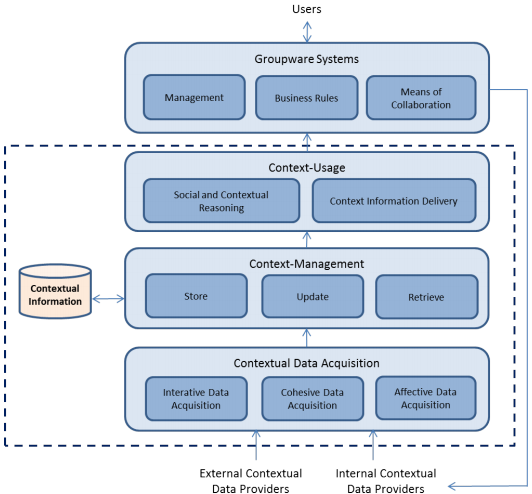
\includegraphics[scale=0.6]{arch}
  \caption{Arquitectura para soportar colaboraci\'on en groupware conscientes del contexto \cite{montane2013context}}
\end{figure}

Muchas arquitecturas se han propuesto para poder soportar sistemas conscientes del contexto, la siguiente tabla hace una comparaci\'on de los elementos y capas de algunas arquitecturas conscientes del contexto, entre las cuales se encuentran la arquitectura base para el presente trabajo que usa un modelo contextual colaborativo clasificado en tres categor\'ias: elementos cohesivos, elementos interactivos y elementos afectivos. La arquitectura de Dey\cite{dey1999architecture}  usa widgets para la captura de datos contextuales y servicios de agregaci\'on de contexto as\'i como servicios de distribuci\'on y razonamiento contextual. En el marco de trabajo de Kamoun \cite{kamoun2012fadyrcos}  se reconfiguran servicios para adaptarlos a situaciones que cambian din\'amicamente. Decouchant \cite{decouchant2013adapting} divide su arquitectura en tres capas: la capa de espacio de trabajo, la de adaptaci\'on y la de detecci\'on de informaci\'on contextual. Guerman  \cite{guermah2013ontology} que propone una arquitectura orientada a sistemas de aprendizaje electr\'onico. En la figura \ref{cmp:fig} se comparan algunos elementos que poseen dichas arquitecturas, entre ellos se encuentran la presencia de capas como adquisici\'on, manejo y distribuci\'on de datos contextuales, persistencia de datos y su reuso, apoyo con v\'ias de comunicaci\'on, el uso de widgets como comunicadores entre el sistema y la arquitectura, manejo de sesiones, esquemas conceptuales de colaboraci\'on, agregaci\'on de datos y la representaci\'on de espacios de trabajo como parte de la arquitectura.

\begin{figure}[h!]
  \centering
    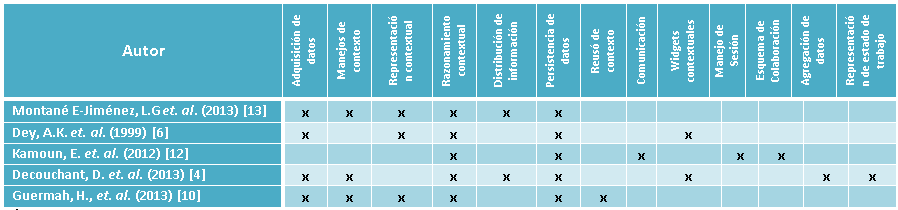
\includegraphics[scale=0.7]{images/comparaciones.png}
  \caption{Comparaci\'on de arquitecturas que soportan consciencia del contexto\cite{montane2013context}\cite{dey1999architecture}\cite{kamoun2012fadyrcos}\cite{decouchant2013adapting}\cite{guermah2013ontology}}
  \label{cmp:fig}
\end{figure}

Dentro las arquitecturas vistas, se identifica un proceso donde la informaci\'on contextual es tratada desde su adquisici\'on hasta la entrega de resultados a las aplicaciones consumidoras.

\subsection{Proceso}

Para obtener resultados de un conjunto de variables contextuales se establecen 3 pasos ya descritos antes \cite{montane2013context}: recuperar las variables contextuales en un formato legible para la computadora, almacenar, recuperar y actualizar los datos contextuales de una base de datos, e inferir resultados de un conjunto particular de variables asociadas unas con otras para despu\'es distribuirlos.

\subsubsection {Adquisici\'on}
El problema de mantener la consciencia del espacio de trabajo en los groupware gira en torno a la obtenci\'on de informaci\'on \'util m\'as que el c\'omo la utilizan los usuarios \cite{ardissono2012context}. Antunes propone un marco de trabajo para evaluar groupwares \cite{antunes2008structuring}, un enfoque entrada-procesamiento-salida para conceptualizar las relaciones entre el soporte tecnol\'ogico y factores relacionados al comportamiento del grupo y contexto de trabajo. Las variables contextuales son factores importantes para describir el comportamiento del grupo, est\'an clasificadas en 5 categor\'ias generales \cite{antunes2008structuring}: personales, situacionales, estructura del grupo, caracter\'isticas de la actividad o tarea y caracter\'isticas tecnol\'ogicas. Los procesos grupales est\'an definidas como las caracter\'isticas de las interacciones del grupo, incluyendo las decisionales, comunicacionales, e interpersonales. Por \'ultimo este framework eval\'ua los resultados de los procesos grupales afectados por el soporte tecnol\'ogico, incluyendo los relacionados con las actividades y con el grupo en s\'i.

\subsubsection {Manejo de contexto}

Alves \cite{alves2013radiator} propone un mecanismo de agregaci\'on de informaci\'on contextual para mejorar la eficiencia de consumo de recursos de red para aplicaciones conscientes del contexto, para esto se define contexto como un conjunto $( P_{n},t_{n},A_{n} )$, conformado por un grupo de personas $(  P_{1}...P_{n} )$ que en un lapso de tiempo $t$ cumplen con un cierto atributo $A$ compuesto por un nombre y un valor, con esto propone una funci\'on de agregaci\'on $Aggr( A_{c}, {( P_{1},t_{1},A_{1} ),..., ( P_{n},t_{n},A_{n} )})$ en la que se mezclan un conjunto de contextos acontecidos en un lapso de tiempo con un atributo $Ac$ en com\'un tal que para todo atributo $A_{i}$ perteneciente a $A_{1} ... A_{n}$, $Ac$ pertenece a $A_{i}$.

AYPUY es un manejador de recursos creado para ambientes de colaboraci\'on distribuidos.  Almacena diferentes tipos de recursos, como contratos, historias cl\'inicas, objetos de aprendizaje, etc., y garantiza su acceso cumpliendo con los objetos de confidencialidad, seguridad y escalabilidad de los sistemas que lo utilizan. En este framework un recurso est\'a compuesto de un conjunto de atributos $A = { L, D, F }$, donde $L$ describe las caracter\'isticas l\'ogicas generales del recurso (fecha de creaci\'on, autor, tipo de recurso), $D$ establece las caracter\'isticas relacionadas con el dominio (e.g., salud, educaci\'on) al que pertenece el recurso, y $F$ describe las caracter\'isticas f\'isicas de almacenamiento del recurso (e.g., tipo de replicaci\'on, cadena de conexi\'on), as\'i AYPUY establece la estrategia de almacenamiento y acceso, adicionalmente los recursos tienen un conjunto de operadores $O$, que determinan las acciones que se pueden hacer con ellos, y son extensibles para soportar un dominio espec\'ifico.

AYPUY administra los recursos controlando su acceso con espacios de trabajo (ET), crea un ET general al que pertenecen todos los usuarios del sistema siguiendo un rol espec\'ifico, si se requiere la especializaci\'on o modificaci\'on de los roles de acceso a los recursos para todos o un subconjunto de usuarios, se crea otro ET. En un ambiente empresarial, por ejemplo, el ET general representa a la empresa, y un ET1 corresponder\'ia a un departamento y ET1.1 a un proyecto en espec\'ifico.

\subsubsection{Distribuci\'on}
La informaci\'on que se recopila se ocupa de qui\'en est\'a trabajando en un contexto compartido, qu\'e est\'an haciendo, d\'onde est\'an trabajando, cu\'ando ocurren varios eventos, y como suceden esos eventos \cite{ardissono2012context}. La presentaci\'on de informaci\'on consciente es una parte importante de los groupware, Gross\cite{gross2013supporting} menciona los siguientes puntos importantes que se deben de tomar en cuenta al momento de presentar informaci\'on al usuario:
\begin{itemize}
\item La identificaci\'on y el se\'nalamiento de retos sobre la desorganizaci\'on de contenedores de informaci\'on consciente son requerimientos centrales para el apoyar la consciencia.
\item Los sistemas deben de proporcionar sugerencias que los usuarios puedan sobrescribir, ya sea en un momento espec\'ifico o como regla general.
\item La presentaci\'on de informaci\'on de consciencia debe de ser explorada con la participaci\'on del usuario, el tipo de visualizaci\'on de consciencia debe de ajustarse a la necesidad de informaci\'on del usuario y a su contexto.
\item Modelos de consciencia son importantes para estructurar informaci\'on de consciencia
\end{itemize}

Alves \cite{alves2013radiator} propone un modelo gen\'erico para propagaci\'on de contexto (Radiator) y necesidades de privacidad de aplicaciones distribuidas conscientes del contexto, enfocado a mejorar la escalabilidad de las aplicaciones y brindar privacidad de la propagaci\'on de la informaci\'on, adem\'as agrega que la escalabilidad y la privacidad se pueden asegurar retrasando la propagaci\'on de contexto hasta que ciertas condiciones son alcanzadas y entonces agregar los mensajes en niveles sint\'acticos y sem\'anticos, antes de propagar la informaci\'on los datos tienen que tener un nivel de agregabilidad determinado de donde  $CP$ es el contexto actual de una persona $P$ y $C_{x}$ el contexto de alguien m\'as que el sistema quiere propagar a $P$, $G( CP, C_{x} )$ representa que tan agregado debe de estar $C_{x}$ antes de ser transmitido a $P$ , tomando en consideraci\'on el contexto actual de $CP$. Por lo tanto un conjunto de contextos $C_{1}..C_{n}$ es solo propagado a $P$ cuando para todo $i$ perteneciente a $1..n$, $G( CP, C_{i} ) = n$, $n$ siendo un entero. Informalmente la agregabilidad representa el n\'umero de mensajes de contexto que deben de ser retenidos antes de su propagaci\'on, si se define una funci\'on $G$ que siempre regrese 4, el sistema siempre va a agregar cuatro mensajes contextuales antes de propagarlos

En el trabajo de Ardissono \cite{ardissono2012context} se mencionan 2 pol\'iticas dependientes del contexto para el manejo de notificaciones que apoya la selecci\'on de notificaciones para ser entregadas en base a las actividades actuales del usuario en diferentes niveles de granularidad: colaboraci\'on general de la tarea actual del usuario contra tarea llevada a cabo. Estas pol\'iticas son ofrecidas por el framework CONRAD (COntext depeNdent awaReness informAtion Delivery, por sus siglas en ingl\'es). Las 2 pol\'iticas son las siguientes:

\begin{enumerate}
\item el filtro de contexto informa al usuario sobre eventos referentes a los contextos de colaboraci\'on en los que est\'a trabajando e ignora los dem\'as
\item el filtro de tareas es m\'as selectivo y filtra las notificaciones basado en la tarea actual del usuario
\end{enumerate}

Con este framework se reduce el nivel de distracci\'on y la carga de trabajo presentada al usuario al momento de obtener informaci\'on relacionada con su actividad.
El objetivo de su trabajo es proveer a usuarios apoyo automatizado para especificar el tipo de informaci\'on consciente m\'as apropiado basado en la actividad del usuario y ajustar la entrega de las notificaciones y la aplicaci\'on de filtros para preferencias individuales de notificaci\'on.

Para adaptar servicios cooperativos al contexto del usuario, AYLLU \cite{arias2012platform} usa el framework AES que adapta la informaci\'on en diversos contextos. AES funciona de la siguiente manera: una aplicaci\'on env\'ia una consulta inicial a AES para que esta la enriquezca, AES obtiene los perfiles o caracter\'isticas de la aplicaci\'on externa (usuario, contexto, dispositivo, perfiles), e invoca funciones de filtro de acuerdo a los perfiles. El resultado es un conjunto de datos de alta abstracci\'on que es usado para generar una consulta enriquecida que ser\'a devuelta a la aplicaci\'on externa.

El framework AYLLU \cite{arias2012platform} usa un protocolo de comunicaci\'on donde los mensajes son enriquecidos sem\'anticamente, como en un sistema multiagentes. Se basa en la creaci\'on de una serie de agentes que ejecutan protocolos de  comunicaci\'on, que ayudan al usuario a seguir una serie de protocolos de interacci\'on que determinan un servicio cooperativo, cuando un servicio cooperativo se instancia se crea un Agente Manejador de Comunidad (CMA) por medio de un agente de f\'abrica (FA), el usuario cuenta con un agente asistente que muestra las peticiones al usuario para generar respuestas.

\subsubsection{Mecanismos de razonamiento}

Para adaptar los sistemas es necesario reconocer la situaci\'on de los usuarios y saber c\'omo brindarles apoyo, en consecuencia se requiere de una forma de interpretar las interacciones que se est\'an llevando a cabo en la aplicaci\'on con lo que se han propuesto diferentes mecanismos de razonamiento para estos casos.

En el modelo contextual MARS se usa un lenguaje de regulaci\'on para describir escenarios llamado CoRaL\footnote{Collaborative Regulation Language} que toma en cuenta tres aspectos de los escenarios definidos en MARS especificados en las pre y pos condiciones de la interacci\'on: qui\'en puede participar en la interacci\'on, qu\'e objetos pueden ser manipulados, qu\'e rol tiene un actor u objeto durante la interacci\'on y en casos similares, referencias a otros escenarios. Con esto se define el lenguaje CoRaL con la siguiente sintaxis(Cuadro \ref{lan:mars}) descrita en noteaci\'on BNF para gram\'aticas libres de contexto. Siendo E el conjunto de elementos de cadenas de nombres de arenas, actores, familias de actores, familias de objetos, objetos y roles. 

\begin{table}
\label{lan:mars}
\centering
\caption{Lenguaje CoRaL}
\begin{tabular}{|p{5cm}|p{8cm}|}
\hline \textbf{No terminal} & \textbf{Expresi\'on}\\
\hline $\langle sentencia \rangle ::=$ & $\langle expresi\acute{o}n \rangle \langle operador \rangle \langle expresi\acute{o}n \rangle";"$\\
\hline $\langle expresi\acute{o}n \rangle  ::=$ & $\langle palabraReservada \rangle :\{\langle elementos \rangle \}$\\
\hline
$\langle expresi\acute{o}n \rangle  ::=$ & $!\langle palabraReservada \rangle :\{\langle elementos \rangle \}$\\
\hline $\langle operador \rangle  ::=$ & $:: | \rightarrow$\\
\hline $\langle palabraReservada \rangle  ::=$ &  ``Arena" | ``Interacci\'on" | ``Actor" | ``Familia de actor" | ``Familia de Objeto" | ``Objeto" | ``Rol"\\
\hline $\langle elemento \rangle  ::=$ & $cualquier cadena en E$ \\
\hline
\end{tabular}
\end{table}

Skillen \cite{Skillen201497} en su capa de uso de contexto define cuatro funciones para el procesamiento de contexto, estas funciones se definen con el lenguaje de reglas de web semantico SWRL con el que describe condiciones que la informaci\'on contextual debe de cumplir para personalizar un conjunto de servicios. Haciendo uso de la sintaxis de este lenguaje definen reglas como la siguiente. 

\textbf{UserProfile(?up), hasHealthCondition(?up, Blind) $\rightarrow$ HelpDelivery(PlayAudio), hasMediaType(PlayAudio, Audio), hasMediaVolumeLevel(PlayAudio, VolLevel\_5)}. 

En la definici\'on se puede observar un caso en el que se especifica la preferencia de audio con un vol\'umen espec\'ifico para la entrega de informaci\'on para una persona con discapacidad visual.

As\'i mismo Bo Hu \cite{bohu2013} implementa el lenguaje SWRL para definir reglas en la ontolog\'ia contextual, estas reglas son una clase de restricciones, relaciones y atributos que se deben de cumplir y siguen una estructura de l\'ogica de predicados. Como ejemplo muestran una regla de ejecuci\'on entre los conceptos de persona y actvividad defini\'endola de la siguiente manera $\forall x.Activity(x) \rightarrow (\sharp \{y|Person(y)\wedge Executing(x,y)\} \geq 1$.

%En el caso de Pereira et. al. \cite{pereira2013CSCWD} el mecanismo de inferencia que implementa es un lenguaje basado en SQL llamado SPARQL el cual realiza consultas sobre ontolog\'ias

En algunos casos se puede notar en los mecanismos de uso de contexto que se hace uso de lenguajes formales para la descripci\'on de situaciones de los usuarios, algunos de ellos se centran en un usuario y lo que pasa alrededor de \'el para inferir resultados, en otros se hace m\'as importante el concepto de trabajo colaborativo y los lenguajes que proponen se centran en describir la actividad de todos los usuarios y mezclar aquellos que tienen contextos similares.
%analisis del caso de estudio %
Como se vi\'o anteriormente las arquitecturas o marcos de trabajo que soporten consciencia contextual deben cumplir con ciertos requerimientos \cite{dey1999architecture}, para poder cubrir estas necesidades se necesita que el marco de trabajo sea accesible por el groupware desde cualquier ubicaci\'on, con esto se cubre la distribuci\'on de la arquitectura, as\'i la publicaci\'on de servicios web consumibles desde el sistema colaborativo se vuelve una soluci\'ona este problema, adem\'as de que con estos servicios aumenta la compatibilidad con otro tipo de plataformas al enviar sus mensajes serializados en Json o envueltos en una solicitud SOAP. Con estos servicios se hace posible la recepci\'on de informaci\'on contextual y la emisi\'on de los resultados hacia el groupware. Con la informaci\'on recivida se mantiene un registro de la actividad del groupware que puede ser \'util para an\'alisis futuros como miner\'ia de datos o reconocimiento de patrones.

La arquitectura no debe de estar enganchada a un escenario en particular, debe de funcionar tanto para un sistema de gu\'ia de turistas como para uno de oficina, es por eso que la definici\'on del modelo contextual se divide en dos partes, un meta modelo compuesto por entidades que describen una actividad mediante realciones de elementos tales como \textit{actores}, \textit{objetos}, \textit{tareas}, \textit{categor\'ias}, \textit{roles}, \textit{comunidades} y \textit{objetivos} con lo que se modela las interacciones del groupware, una vez modelado el dominio del sistema se instancia a partir del meta modelo, es en esta instanciaci\'on donde se guardar\'an los datos del groupware.

Los datos recibidos deben de ser gestionados en bases de datos y procesados por un motor de razonamiento, el cu\'al tiene que recibir informaci\'on contextual y mediante alg\'un proceso tiene que dar como resultado informaci\'on para el usuario o un comando de ejecuci\'on para el groupware. Una vez que se procesa la informaci\'on esta se tiene que preparar para su distribuci\'on en los diferentes dispositivos cliente. Para esto se debe de considerar que al ser las actividades colaborativas los usuarios pueden compartir el contexto en algunas ocasiones, de lo que se desprende la necesidad de agregar la informaci\'on contextual de usuarios que compartan ciertos atributos establecidos para una situaci\'on en particular, es decir, fusionar la informaci\'on de tales usuarios para un manejo de la informaci\'on m\'as eficiente.

\subsection{Caso de estudio}

Para el actual proyecto se necesita un groupware al cu\'al se le pueda acoplar la arquitectura para poder analizar sus datos, en este caso el sistema elegido es un videojuego colaborativo de disparos en primera persona, \textit{AssaultCube}. Este groupware en particular tiene las caracter\'isticas de ser distribuido y s\'incrono seg\'un la clasificaci\'on de Ellis\cite{ellis1991groupware}, contiene varios tipos de elementos y los modos multijugador son entre equipos en los cuales se requiere de una buena colaboraci\'on para cumplir los objetivos de la actividad, El juego cuenta con un servidor y varios clientes que se conect\'an a \'el para poder jugar, la arquitectura tendr\'a que estar acoplada al servidor ya que este es el que recibe toda la informaci\'on de las actividades de los clientes. \textit{Assault Cube} tiene diferentes modos de juego, entre ellos capturar la bandera, cuyo objetivo es llegar a la base enemiga y recuperar la bandera que est\'a ah\'i para regresarla a la propia bas; otro modo de juego es rey de la colina, que tiene por objetivo mantenerse m\'as tiempo en una posici\'on marcada por el juego que el equipo contrario; hay m\'as formas de juego adem\'as de estas dos, y en cada una de ellas las actividades son diferentes y poseen objetivos diferentes, sin embargo pueden compartir interacciones como eliminar a un enemigo por ejemplo.

\begin{figure}[h!]
\centering
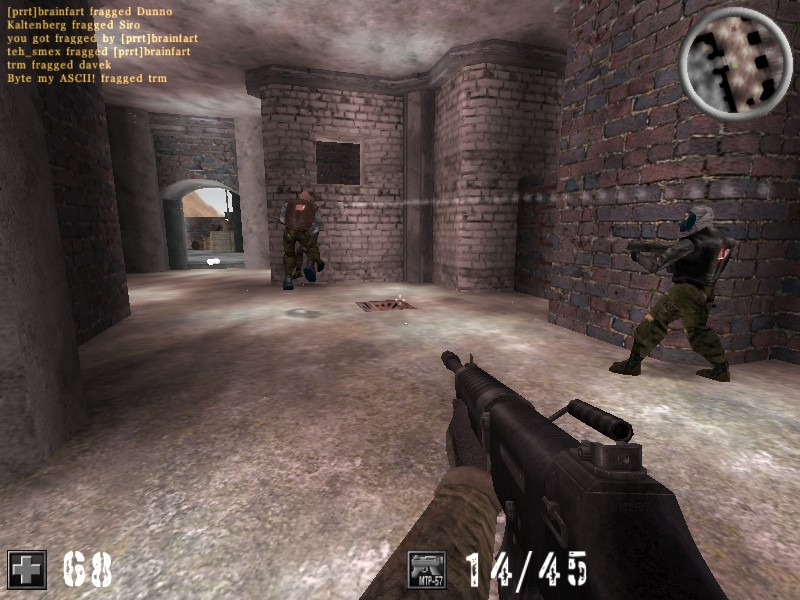
\includegraphics[scale=.15]{images/assaultcube}
\caption{Assault Cube}
\label{gw:asscb}
\end{figure}

En la Tabla 1 se muestran las interacciones identificadas en el juego para la actividad relacionada al modo de juego de capturar la bandera, estas interacciones est\'an relacionadas directamente con las actividades que se pueden llevar a cabo en el groupware, las interacciones se vuelven irrelevantes cuando no tienen conexi\'on con ninguna actividad, por ejemplo las interacciones del usuario con elementos de configuraci\'on en este caso particular, como en la interacci\'on \textit{"Jugador elige modo de juego"}. En estas interacciones se encuentran algunos elementos del modelo como pueden ser Actores, Tareas y Objetos,  esto nos da la pauta para empeazar a dise\~nar nuestro modelo.

\begin{center}
\label{AC:interacciones}
\begin{longtable}{|p{5cm}|p{7cm}|}

\caption{Tabla de interacciones detectadas en \textit{Assault Cube}}\\
\hline
\textbf{Interacci\'on} & \textbf{Elementos identificados}\\
\hline
\endfirsthead
\multicolumn{2}{c}%
{\tablename\ \thetable\ -- \textit{... Contin\'ua de p\'agina anterior}} \\
\hline
\textbf{Interacci\'on} & \textbf{Elementos identificados} \\
\hline
\endhead
\hline \multicolumn{2}{r}{\textit{Contin\'ua en siguiente p\'agina...}} \\
\endfoot
\hline
\endlastfoot
\textbf{Jugador se Mueve} & Actor: Jugador; Tarea: Moverse\\\hline

\textbf{Jugador salta} & Actor: Jugador; Tarea: Saltar\\\hline

\textbf{Jugador dispara arma} & Actor: Jugador; Tarea: Saltar; Objeto: Arma\\\hline

\textbf{Jugador recarga arma} & Actor: Jugador; Tarea: Recargar; Objeto: Arma\\\hline

\textbf{Jugador dispara arma} & Actor: Jugador; Tarea: Saltar; Objeto: Arma\\\hline

\textbf{Jugador cambia arma} & Actor: Jugador; Tarea: Cambiar; Objeto: Arma\\\hline

\textbf{Jugador obtiene mejora de salud} & Actor: Jugador; Tarea: Obtener; Objeto: Mejora de salud\\\hline

\textbf{Jugador obtiene protecci\'on} & Actor: Jugador; Tarea: Obtener; Objeto: Protecci\'on\\\hline

\textbf{Jugador obtiene munici\'on} & Actor: Jugador; Tarea: Obtener; Objeto: munici\'on\\\hline

\textbf{Jugador envia mensaje de texto} & Actor: Jugador; Tarea: enviar; Objeto: Mensaje de texto\\\hline

\textbf{Jugador envia mensaje de voz predefinido} & Actor: Jugador; Tarea: enviar; Objeto: Mensaje de voz\\\hline

\textbf{Jugador elige arma inicial} & Actor: Jugador; Tarea: Elegir; Objeto: Arma predeterminada\\\hline

\textbf{Jugador cambia rol} & Actor: Jugador; Tarea: Cambiar; Objeto: Rol\\\hline

\textbf{Jugador se agacha} & Actor: Jugador; Tarea: Agacharse\\\hline

\textbf{Jugador se suicida} & Actor: Jugador; Tarea: Suicidarse\\\hline

\textbf{Jugador es eliminado} & Actor: Jugador; Tarea: Ser eliminado\\\hline

\textbf{Jugador elimina oponente} & Actores: JugadorA, JugadorB; Tarea: Eliminar\\\hline

\textbf{Jugador reaparece} & Actor: Jugador; Tarea: Reaparecer\\\hline

\textbf{Jugador captura bandera} & Actor: Jugador; Tarea: Capturar; Objeto: Bandera\\\hline

\textbf{Jugador regresa bandera a su base} & Actor: Jugador; Tarea: Recuperar; Objeto: Bandera \\\hline

\textbf{Jugador ve mapa} & Actor: Jugador; Tarea: Ver; Objeto: Mapa\\\hline

\textbf{Jugador ve puntuaciones} & Actor: Jugador; Tarea: Ver; Puntuaciones\\\hline

\end{longtable}
\end{center}

En la lista anterior se pueden identificar ya algunos elementos del modelo del groupware, por ejemplo, jugador como actor; arma, munici\'on y mapa como posibles objetos, y el conjunto de ellos relacionados con una acci\'on como tareas. Tambi\'en a partir de estas interacciones pueden empezar a definirse algunas reglas, por ejemplo establecer una regla que diga que si un jugador captur\'o una bandera y est\'a en peligro inminente de ser atacado, el sistema muestre a sus compa\~neros de equipo la ubicaci\'on del abanderado y env\'ie una se\~nal de auxilio para que ellos puedan acudir a su ayuda.

En las reglas definidas para describir el contexto se muestran tres tipos diferentes:

\begin{itemize}
\item Pertenencia(P): Estas reglas verifican si un elemento est\'a contenido o relacionado con otro. Esta regla est\'a definida por $Elemento [ \rightarrow | \rightsquigarrow ] Elemento$; por ejemplo la pertenencia de un actor a un equipo determinado.
\item Comparaci\'on(C): comparan el atributo  de un elemmento con un valor. La sintaxis para esta regla es la siguiente $Elemento.NombreAtributo [ = | ¬ | < | > ] Valor$; por ejemplo que el nombre de un jugador sea "Jes\'us".
\item Ejecuci\'on(X): indica que una tarea ha sido llevada a cabo, y si es el caso, con qu\'e objeto se realiz\'o, adem\'as se puede puntualizar otras caracter\'isticas de la tarea como efectividad, o la afectaci\'on que tuvo, y si es necesario se puede a\~nadir una regla de pertenencia en la misma declaraci\'on del elemento.  $ [Elemento | P] - Task(nombre, Elemento) [ .nombreAtributo [ = | ¬ | < | > ] valor ]$; un ejemplo pr\'actico de esta regla puede ser la ejecuci\'on de un disparo efectivo por parte de un jugador perteneciente al equipo rojo con un francotirador.
\end{itemize}

En donde $Elemento$ es un elemento del modelo, el cual es descrito por un meta elemento, un elemento del modelo, y la instancia o instancias quedando la sintaxis de la siguiente forma: $MetaElemento(Elemento{ListaDeInstancias})$, evidentemente los elementos y lsa instancias tienen que formar parte del modelo. As\'i se cre\'o la siguiente gram\'atica libre de contexto que es la que valida el correcto uso de este lenguaje:
\begin{itemize}
\item $S \rightarrow ML:=XJ$
\item $M \rightarrow P$
\item $M \rightarrow C$
\item $M \rightarrow X$
\item $J \rightarrow \&XJ$
\item $J \rightarrow \lambda$
\item $L \rightarrow \&ML$
\item $L \rightarrow \lambda$
\item $E \rightarrow m(e{iH})$
\item $E \rightarrow m(*)$
\item $E \rightarrow m(e{*})$
\item $E \rightarrow m(iH)$
\item $H \rightarrow ,iH$
\item $H \rightarrow \lambda$
\item $P \rightarrow EOE$
\item $O \rightarrow \Rightarrow$
\item $O \rightarrow \rightsquigarrow$
\item $C \rightarrow E.aKv$
\item $K \rightarrow =$
\item $K \rightarrow ¬$
\item $K \rightarrow <$
\item $K \rightarrow >$
\item $X \rightarrow F-t(n,F)Q$
\item $X \rightarrow F-t(n)Q$
\item $Q \rightarrow .aKv$
\item $Q \rightarrow \lambda$
\item $F \rightarrow E$
\item $F \rightarrow [P]$
\end{itemize}


Con estas interacciones y el conjunto de reglas definido se propone un conjunto de guiones que describen diferentes tipos de comportamiento dado el caso de estudio; entre los que se encuentra un guion para jugadores novatos, un guion para jugadores in\'utiles, uno para jugadores con comportamiento sospechoso que podr\'ian considerarse como traidores y uno para jugadores expertos. Estos guiones servir\'an al momento de ejecutar el sistema \textit{AssaultCube} se estar\'a recibiendo tareas ejecutadas durante las partidas, estas tareas ser\'an comparadas con cada uno de los guiones y se contar\'a la frecuencia de cada una de ellas, cuando las ejecuciones lleguen a el n\'umero indicado, el guion se cumplir\'a y se mandar\'a otra tarea como resultado para que se ejecute en el groupware. Una vez que se cumple un guion, este se reinicia para continuar recibiendo las tareas desde el sistema. Los guiones se definen como sigue.

\textbf{Guion para jugador in\'util:}

$Actor(Player{*})-Task(Shot) [<3]\\
\& Actor(Player{*})-Task(Move) [>10] \\
\& Actor(Player{*})-Task(PickItem) [>5]\\ 
\& Actor(Player{*}).Attribute(enemyKills)=0 \\
\& Actor(Player{*}).Attribute(allyKills)=0\\
\& Actor(Player{*})-Task(captureFlag) [=0]\\
\& Actor(Player{*}).Attribute(socialPresense)=bad\\
\& Actor(Player{*}) \rightarrow Team(red)\\
:= 
[Actor(Player{*})  \rightarrow Team(red)]-Task(sendWarningMessage"Someone is playing fool"), Object(UI{messageConsole})$

\textbf{Guion para jugador novato:}

$
Actor(Player{*}).Attribute(enemyKills)<2\\
\& Actor(Player{*}).Attribute(deads)>2\\
\& Actor(Player{*})-Task(Shot) [>5]\\
\& Actor(Player{*})-Task(scoreCapturedFlag) [<1]\\
\& Actor(Player{*})-Task(loseFlag) [>1]\\
\& [Actor(Player{*}) \rightarrow Team(red)]-Task(Shot).Success = true [<5]\\
\& [Actor(Player{*}) \rightarrow Team(red)]-Task(Shot).Dimension = positive [<5]\\
:=
[Actor(Player{*}) \rightarrow Team(red)]-Task(sendMessage"Noob Player needs help", Object(UI{messageConsole})$

\textbf{Guion para jugador experto:}

$
Actor(Player{*}).Attribute(enemyKills)>5\\
\& [Actor(Player{*}) \rightarrow Team(red)]-Task(Shot).Success = true [>5]\\
\& [Actor(Player{*}) \rightarrow Team(red)]-Task(Shot).Dimension = positive [>5]\\
\& [Actor(Player{*}) \rightarrow Team(red)]-Task(Destroy).Bearer = true [>0]\\
\& Actor(Player{*})-Task(captureFlag)[>3]\\
\& Actor(Player{*}).Attribute(socialPresence)=quite good\\
\& Actor(Player{*}).Attribute(deads)<2\\
:=
[Actor(Player{*}) \rightarrow Team(red)]-Task(showPosition,Object(UI{map,displayScreen})\\
\& [Actor(Player{*}) \rightarrow Team(red)]-Task(sendHelpMessage"stayCloseToHero",Object(UI{messageConsole})
$

\textbf{Guion de jugador traidor:}

$
Actor(Player{*})-Task(captureFlag)[=0]\\
\& [Actor(Player{*})->Team(red)]-Task(Shot)-Affects([Actor(Player{*})->Team(red)]) [>3]\\
\& Actor(Player{*}).Attribute(socialPresence) = bad\\
\& Actor(Player{*}).Attribute(allyKills) > 2\\
\& [Actor(Player{*})->Team(red)]-Task(Shot).Dimension = negative [>5]\\
\& [Actor(Player{*})->Team(red)]-Task(Shot).Dimension = positive [=0]\\
:=
[Actor(Player{*})->Team(red)]-Task(blockWeaponry)-Affects([Object(Weapon{*})->Actor(Player{*})])\\
\& [Actor(Player{*})->Team(red)]-Task(sendWarningMessage"there is a traitor in our lines",Object(UI{messageConsole})
$

\subsection{Prototipo}
Para el presente trabajo se hace uso de un meta modelo contextual para el modelado de actividades de sistemas groupware basado un modelo propuesto anteriormente\cite{montane2013context}, en el cual se pueden encontrar dos categor\'ias de elementos, interactivos y cohesivos.  Entre los interactivos se encuentran \textit{actores}, que son los usuarios del sistema, \textit{objetos} que se usan en \textit{tareas} o que son producto de ellas, \textit{categor\'ias} que clasifican a los actores, objetos y tareas seg\'un sus atributos, por \'ultimo est\'an los roles del objeto y del actor los cuales son asignadas a una tarea para establecer el rol que va a tener el actor u objeto involucrado en dicha tarea. Entre los datos cohesivos se encuentran las \textit{comunidades} que son el conjunto de actores con una \textit{actividad} en com\'un, estas actividades pueden tener varias \textit{metas} las cuales se cumplen realizando tareas. Por \'ultimo se encuentran las reglas que son sentencias en un lenguaje definido para poder inferir las interacciones que suceden en el groupware. En la figura \ref{cmp:mmc} se muestra un diagrama de los elementos de este modelo y sus relaciones.

\begin{figure}[h!]
  \centering
    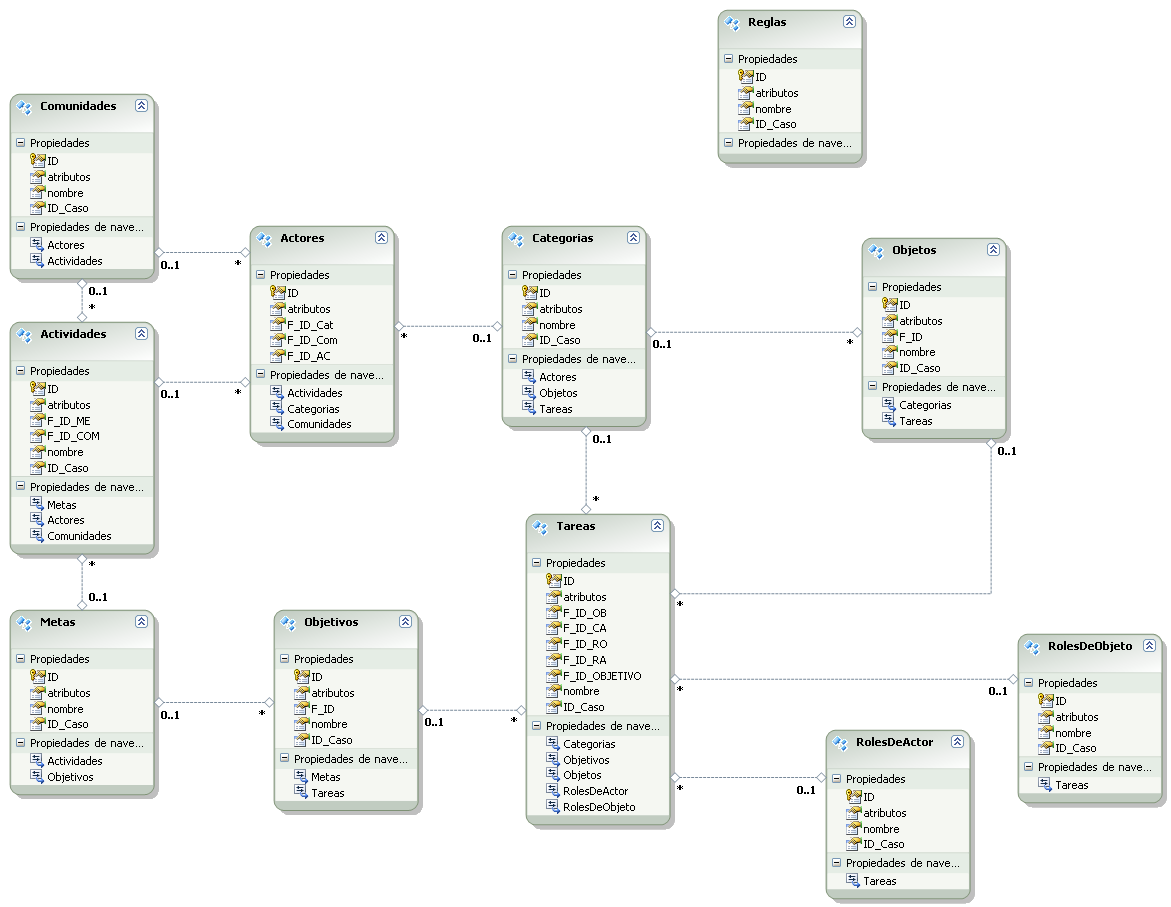
\includegraphics[scale=0.35]{images/modelo}
  \caption{Meta modelo contextual}
  \label{cmp:mmc}
\end{figure}

Con este meta modelo contextual se pueden describir groupwares definiendo cada uno de estos elementos a partir de interacciones, una vez dado de alta un caso junto con sus reglas se instancia un modelo que representar\'a al sistema colaborativo y almacenar\'a las variables contextuales que este transmita a la arquitectura. Cabe mencionar que en este metamodelo los elementos cuentan con 3 atributos principales, un identificador del objeto, un nombre descriptivo, y una lista de atributos almacenados en formato JSON, lo que vuelve flexible la forma de registrar casos de estudio.

La arquitectura que se propone mostrada en la figura \ref{ARCH:propuesta}, cuenta con tres capas: recuperaci\'on de datos, gesti\'on de contexto, y uso de contexto. Para poder acoplar la arquitectura primero se tiene que dar de alta un modelo del groupware. Para esto se cre\'o una plataforma para registrar casos de estudio en la que se establece el nombre del caso de estudio y todos sus elementos, una vez creado el meta modelo del groupware se instancia el modelo y se administran las interacciones para poder relacionar sus elementos, esto se hace en una segunda plataforma en la que se toman los elementos del meta modelo y se instancia uno m\'as apegado al groupware, ya con este modelo se pueden capturar los datos contextuales que el sistema va a enviar a la arquitectura. 

\begin{figure}[h!]
\centering
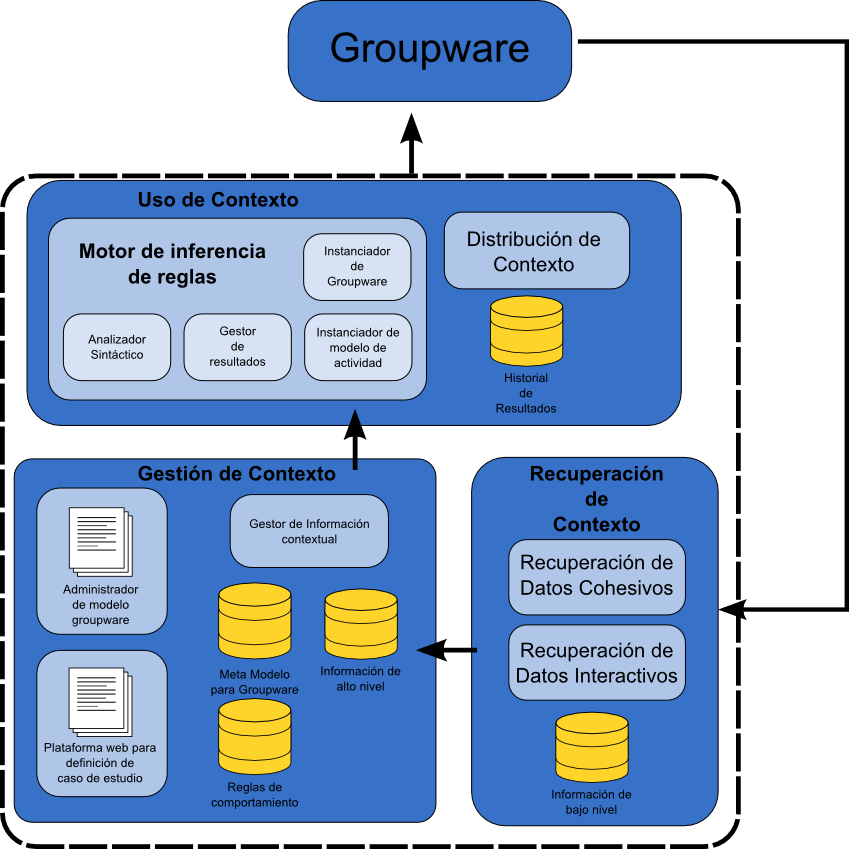
\includegraphics[scale=0.40]{images/arch2}
\caption{Arquitectura propuesta}
\label{ARCH:propuesta}
\end{figure}

La arquitectura, similar a la arquitectura en que se bas\'o, se divide en tres capas; la capa de recuperaci\'on de datos, la capa de gestion de datos y la capa de uso de contexto. En la primera capa, la de recuperac\'on de datos, se captura informaci\'on contextual enviada por el groupware por medio de servicios web publicados para la comunicaci\'on entre la arquitectura y el sistema, estos datos son enviados en un formato espec\'ifico para que capas superiores puedan procesarla. Seguido de este m\'odulo est\'a el degesti\'on contextual, este gestor se encarga de registrar, actualizar y recuperar la informaci\'on contextual en bases de datos, es a este nivel donde el meta modelo y el modelo del sistema se elaboran y donde los datos enviados desde el groupware se registran y son recuperados para inferir resultados en niveles superiores.

En esta capa se encuentra una plataforma en la que se pueden dar de alta elementos del modelo de actividad.

En la \'ultima secci\'on de la arquitectura, uso de contexto, los datos contextuales recuperados son procesados por un motor de inferencia que da como resultado informaci\'on de inter\'es para los usuarios o comandos de ejecuci\'on para la adaptaci\'on del sistema a la situaci\'on actual. El nucleo de este motor es un aut\'omata que especifica un lenguaje para definir reglas, mismas que van a ser definidas en las plataformas antes mencionadas, dentro del motor se har\'a una instancia del modelo del groupware con los datos que env\'ie el sistema, as\'i se puede comparar su estado actual con las reglas de inferencia con el objetivo de ofrecer resultados coherentes al tiempo en el que el sistema se ejecuta. Los resultados obtenidos son gestionados por un administrador de resultados que almacena los datos en una base de datos para mantener registro hist\'orico del comportamiento del groupware. Una vez obtenidos y almacenados los resultados un m\'odulo de distribuci\'on de datos se encarga de enviar la informaci\'on al groupware con la informaci\'on de entrega necesaria. Este proceso es iterativo, ya que vive por el tiempo en el que el groupware opera.
\newpage
%IEEE
\bibliographystyle{IEEEtran}
%\bibliographystyle{apalike}
%\bibliographystyle{apacite}
\bibliography{biblio/biblio}
\end{document}